% vim: filetype=tex spell 

%CubeSat Chapter 
\chapter{Hardware Implementation of the \acf{ACDS}}\label{ch:CubeSatHardware}

As stated in \cref{ch:BG} the system design from \cite{Mentch11} has been modified for the implementation in this thesis. The only hardware change from \cite{Mentch11} is to use four alnico1 torquers in each axis instead of two alnico1 and two vernier torquers as proposed. This does not effect the electrical hardware as both torquer types are the same size and are flipped by the same circuit.

The \ac{ACDS} board for the \ac{ARC} only contains the processor, torquers and drivers. The sensors are located off board and managed by the \ac{LEDL}. The sensor data is sent over the bus to the \ac{ACDS} processor. 

%Both the  \ac{LPMT} and the biasing algorithm have never been flight tested. To test the \ac{LPMT} and bias algorithm the \ac{ARC} will fly an \ac{ACDS} that uses \acp{LPMT}. The central \ac{ACDS} processor and the hardware required to flip the torquers are located on the \ac{ACDS} board while the sensors are located on the \acp{SPB}.

\section{Mechanical Configuration of the \acf{ARC}}

\Cref{fig:arcMech} shows the mechanical design of the \ac{ARC}. The design has a central board stack with solar panels and rails attached to rings that are on the top and bottom of the board stack. The boards in the stack are connected by a 104-pin stack through header that is located on the -Y edge of each board. The header distributes power and allows for communication between boards. 

\begin{figure}[!ht]
    \centering
    \begin{minipage}{0.31\linewidth}
        \begin{tikzpicture}[remember picture,node distance=1em]
            \def\sysx{0.8}
            \node[anchor=south west,inner sep=0] (image) at (0,0) {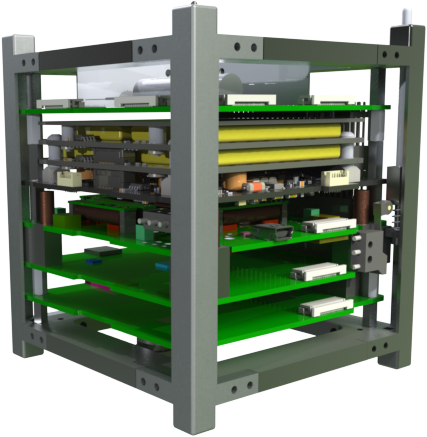
\includegraphics[width=\linewidth]{cubesat-core}};
            \begin{scope}[x={(image.south east)},y={(image.north west)}]
                % define destination coordinates
                \path (\sysx,0.751) coordinate (LEDL)
                      (\sysx,0.633) coordinate (EPS)
                      (0.86,0.55) coordinate (Z1tq)
                      (0.12,0.55) coordinate (Z2tq)
                      (0.3,0.52) coordinate (Xtq)
                      (\sysx,0.465)  coordinate (ACDS)
                      (0.9,0.4)  coordinate (sep)
                      (\sysx,0.366)  coordinate (COMM)
                      (\sysx,0.281)  coordinate (IMG);
              %draw axis
                \path (0.1,0.12) coordinate (axOrig);
                \draw[->,blue,very thick] (axOrig) to +(-21:0.1) coordinate (X);
                \node[blue,right of=X] (Xl) {X};
                \draw[->,magenta,very thick] (axOrig) to +(196:0.1) coordinate (Y);
                \node[magenta,left of=Y] (Yl) {Y};
                \draw[->,red,very thick] (axOrig) to +(-90:0.1) coordinate (Z);
                \node[red,below of=Z] (Zl) {Z};
              \end{scope}
        \end{tikzpicture}
    \end{minipage}\begin{minipage}{0.65\linewidth}
        \begin{itemize}\setlength{\parskip}{0pt}
            \item[\kern-2em] \tikz[na] \coordinate (LEDLi); \acf{LEDL}
            \item[\kern-2em] \tikz[na] \coordinate (EPSi); \acf{EPS}
            \item[\kern-2em] \tikz[na] \coordinate (ACDSi); \acf{ACDS}
            \item[\kern-2em] \tikz[na] \coordinate (sepi); Separation switch
            %\item[\kern-2em] \tikz[na] \coordinate (ppi); Pull Pin
            \item[\kern-2em] \tikz[na] \coordinate (COMMi); \acf{COMM}
            \item[\kern-2em] \tikz[na] \coordinate (IMGi); \acf{IMG}
        \end{itemize}
    \end{minipage}

    \begin{tikzpicture}[overlay,remember picture]
            \path[->,red,very thick] (LEDLi) edge (LEDL);
            \path[->,red,very thick] (EPSi) edge (EPS);
            \path[->,red,very thick] (ACDSi) edge (ACDS);
            \path[->,red,very thick] (sepi) edge (sep);
            \path[->,red,very thick] (COMMi) edge (COMM);
            \path[->,red,very thick] (IMGi) edge (IMG);
            %draw axis
    \end{tikzpicture}
    \caption{The \acs{ARC} mechanical setup}
    \label{fig:arcMech}
\end{figure}

The \ac{ACDS} board is located 3rd from the bottom of the stack. This puts it in the center of the board stack. Because the solar cells cover all of the side faces except a small strip in the center this makes the \ac{ACDS} board the only place to put the pull pin and \ac{USB} connector, that need to be accessed while \ac{ARC} is in the \ac{PPOD}. The separation switch connections are also located on the \ac{ACDS} board, as the separation switch is attached to one of the torquer standoffs.

\begin{figure}[!ht]
    \centering
    \begin{minipage}{0.30\linewidth}
        \centering\large{Back}
        \begin{tikzpicture}[remember picture] 
            \node[anchor=south west,inner sep=0] (image) at (0,0) {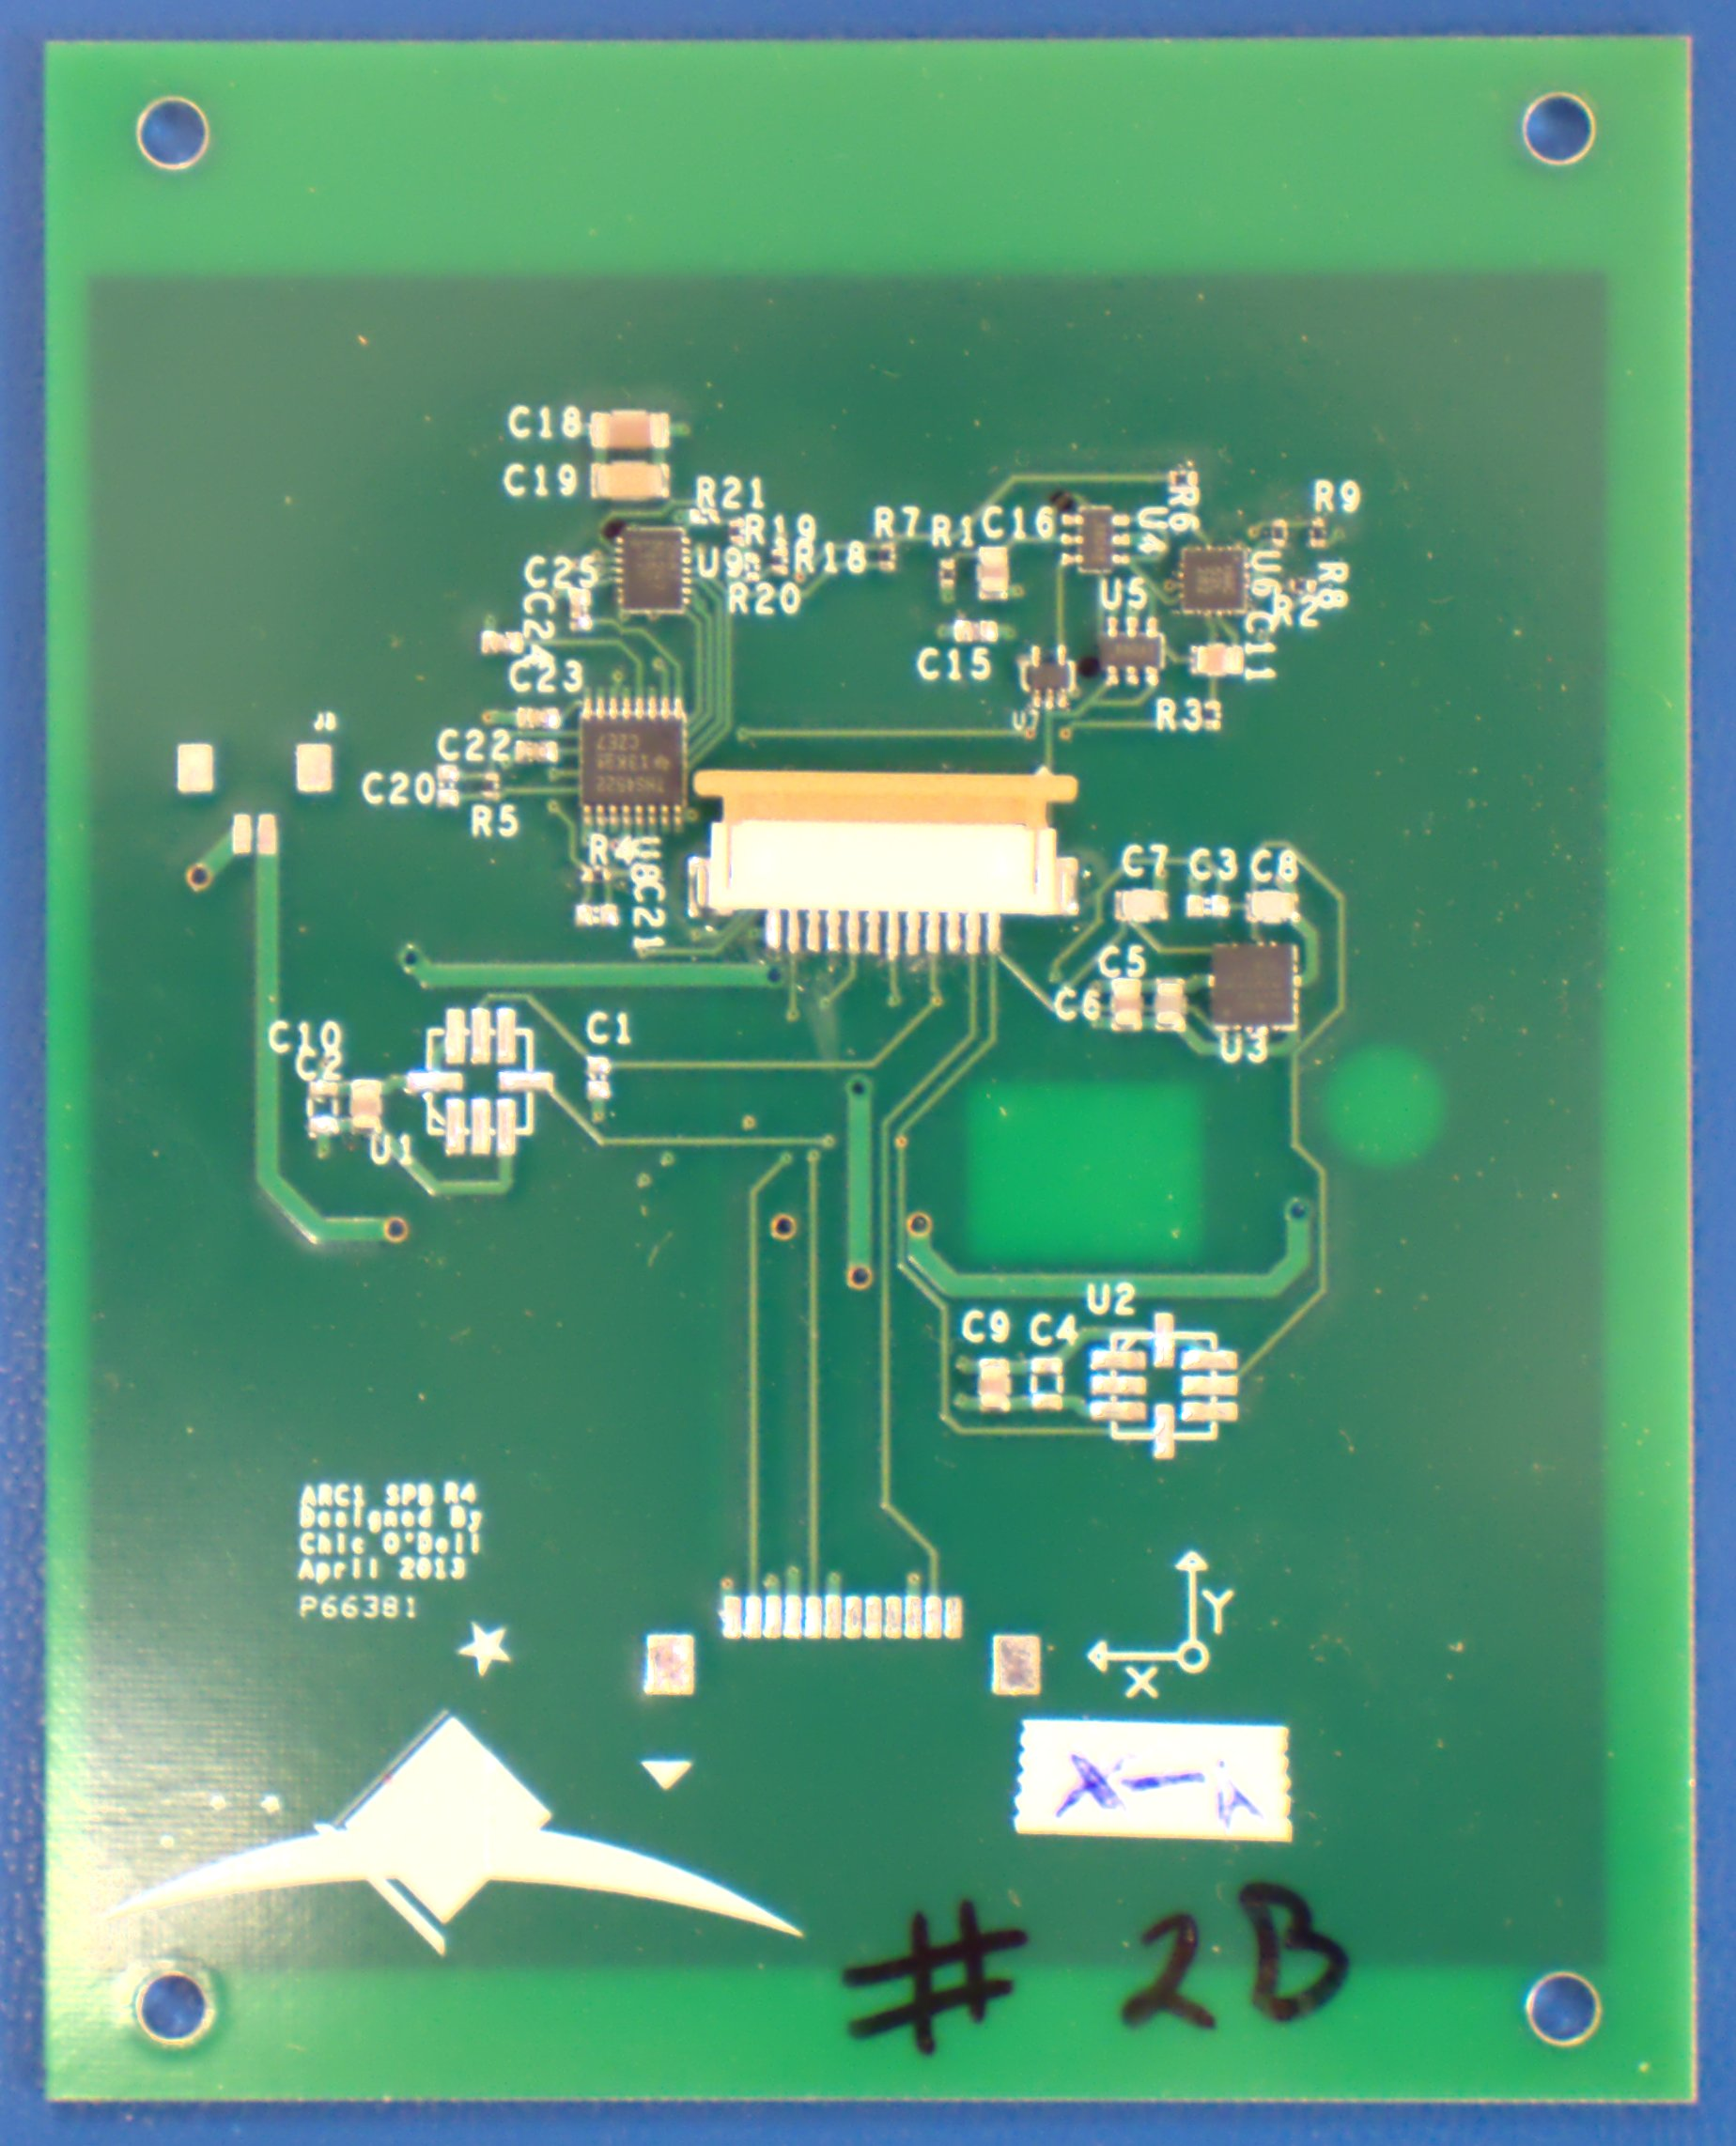
\includegraphics[width=\linewidth]{SPB-back}};
            \begin{scope}[x={(image.south east)},y={(image.north west)}]
                \path (0.715,0.74) coordinate (MAG)
                      (0.395,0.72) coordinate (ADC)
                      (0.395,0.65) coordinate (AMP)
                      (0.745,0.525) coordinate (ACC)
                      (0.615,0.58) coordinate (DAT);
              \end{scope}
        \end{tikzpicture}
    \end{minipage}\begin{minipage}{0.30\linewidth}
        {\large\vspace{1.5em}}
        \vspace*{\fill}
        \begin{itemize}\setlength{\parskip}{0pt}
            \item[\kern-0.2em] Temperature Sensor \tikz[na] \coordinate (TEMPi);
            \item[\kern-0.2em] \tikz[na] \coordinate (MAGi); Magnetometer
            \item[\kern-0.2em] \tikz[na] \coordinate (ADCi); \acs{ADC}
            \item[\kern-0.2em] \tikz[na] \coordinate (AMPi); Amplifier
            \item[\kern-0.2em] Solar Cells \tikz[na] \coordinate (SCi);
            \item[\kern-0.2em] \tikz[na] \coordinate (ACCi); Accelerometer
            \item[\kern-0.2em] \tikz[na] \coordinate (DATi); Data Connector
        \end{itemize}
        \vspace*{\fill}
    \end{minipage} \begin{minipage}{0.30\linewidth}
        \centering\large{Front}
        \begin{tikzpicture}[remember picture] 
            \node[anchor=south west,inner sep=0] (image) at (0,0) {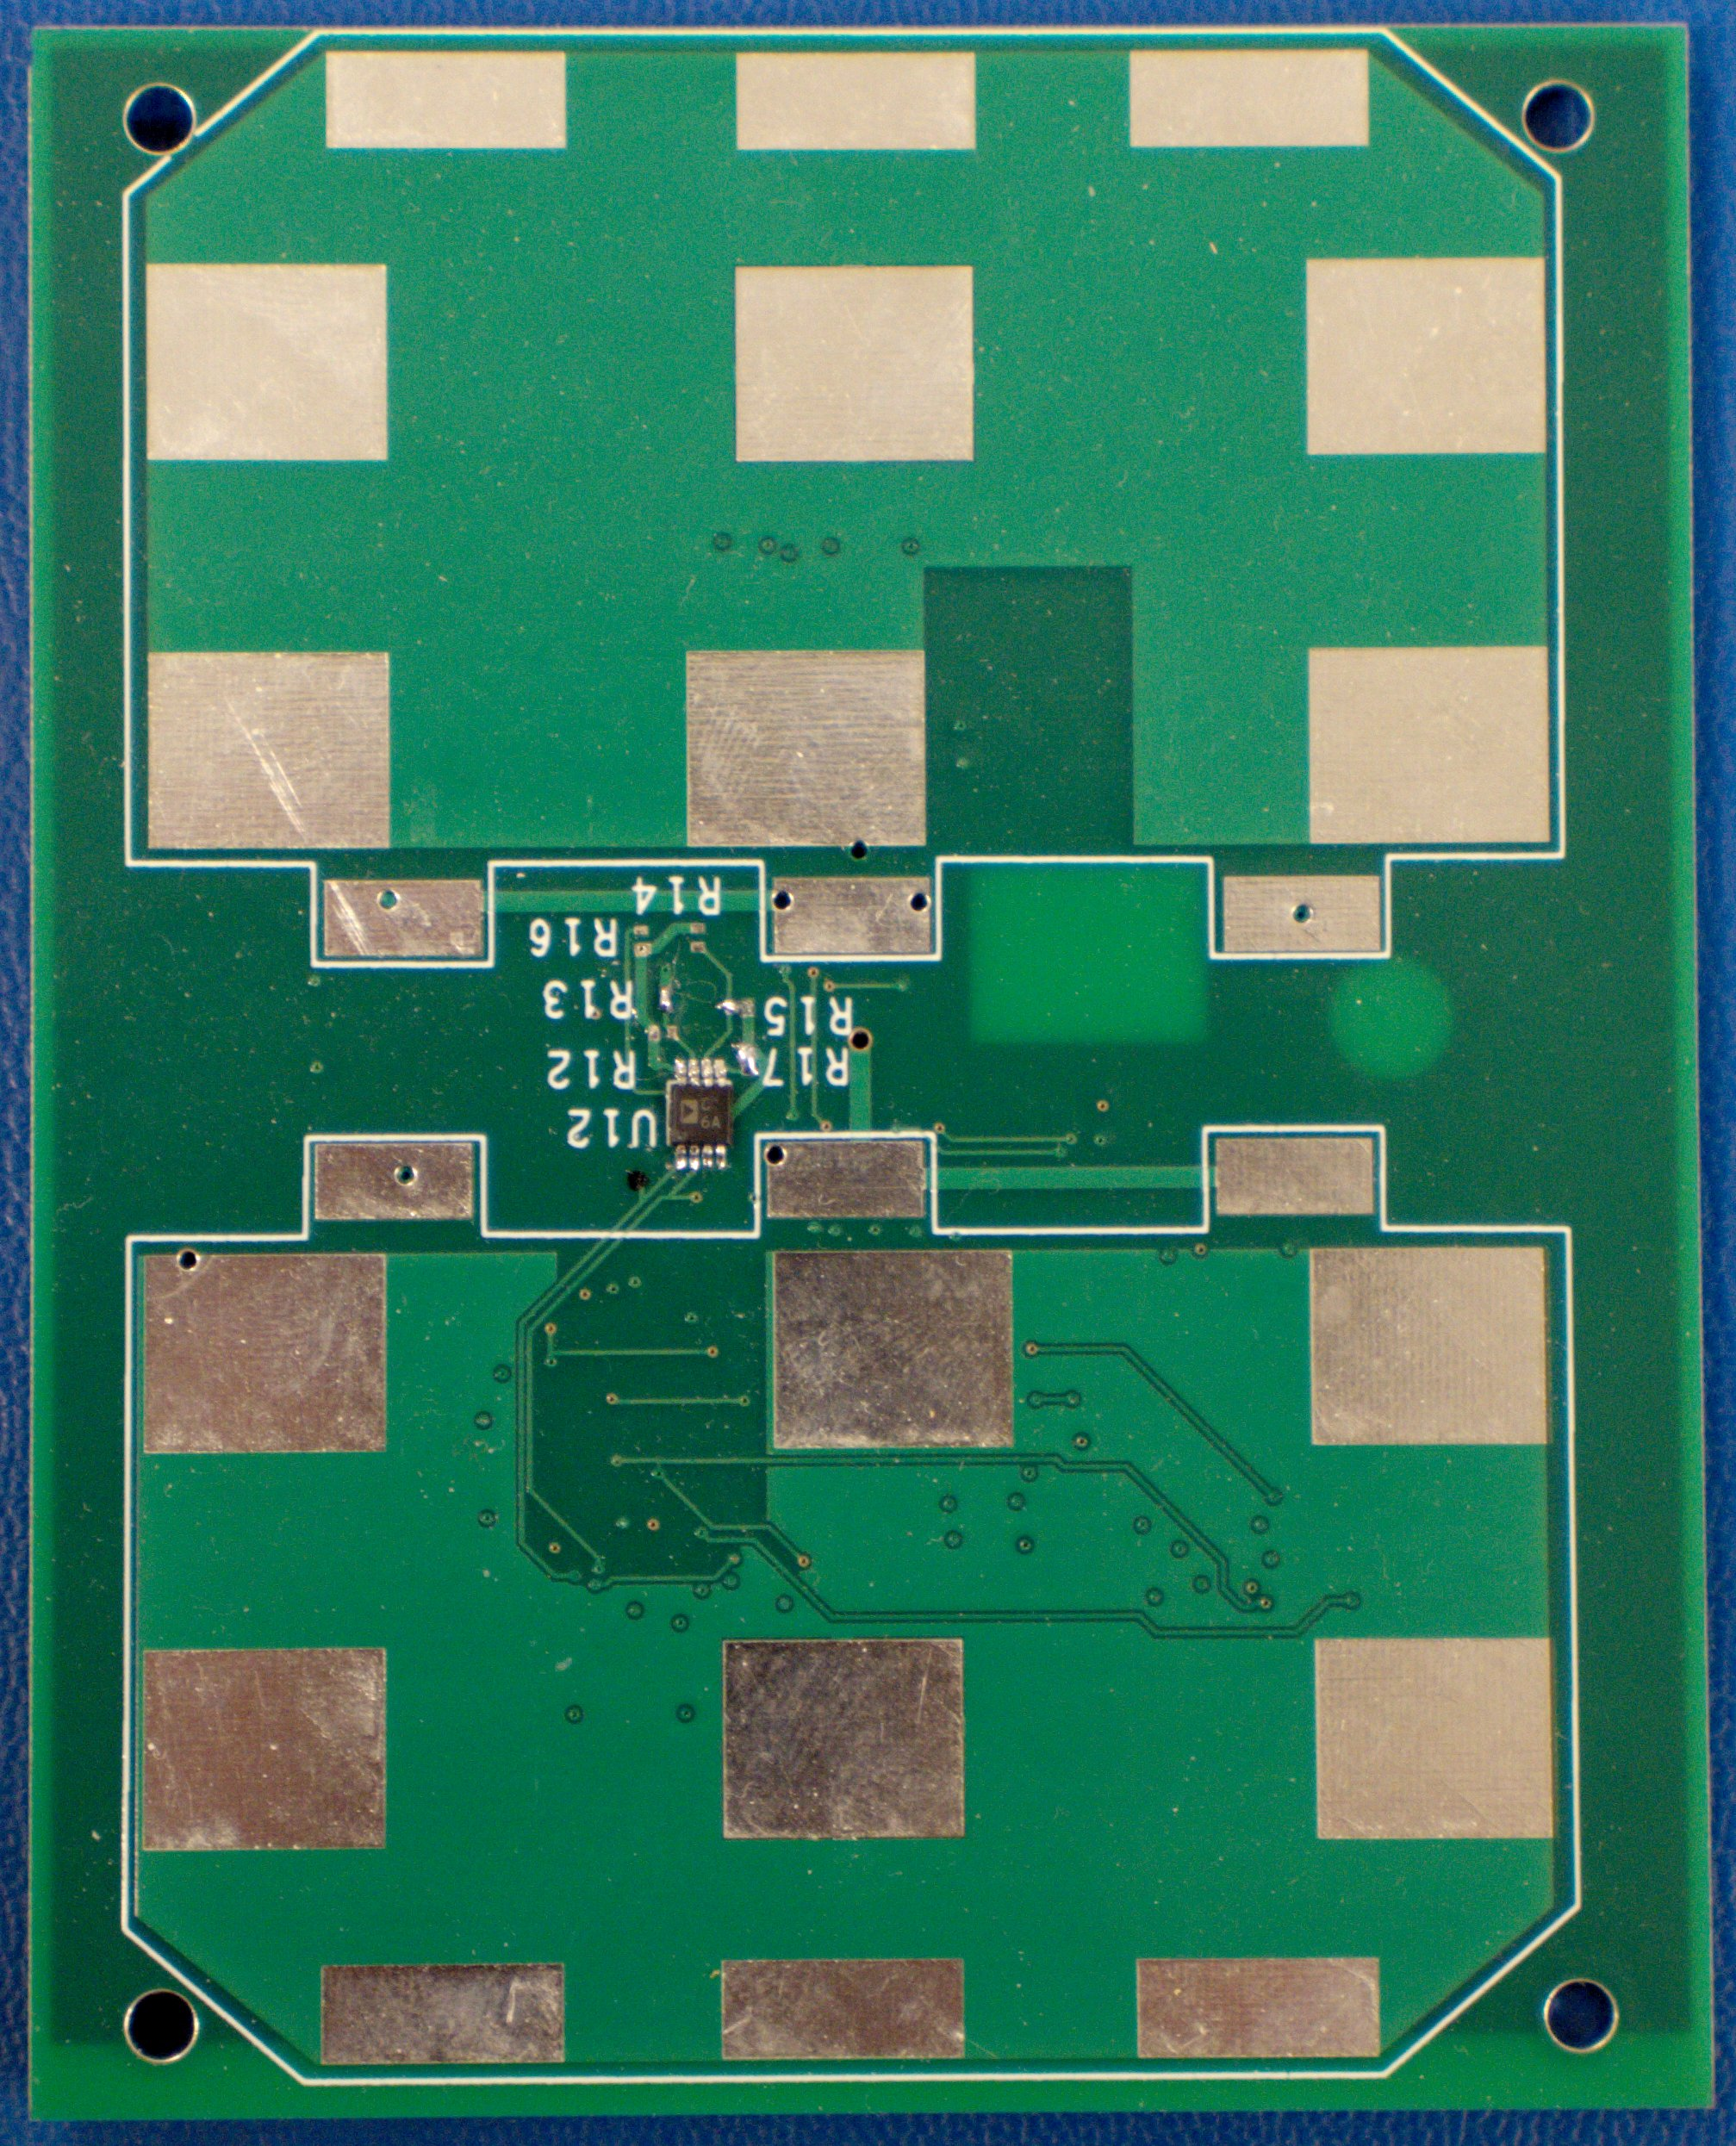
\includegraphics[width=\linewidth]{SPB-front}};
            \begin{scope}[x={(image.south east)},y={(image.north west)}]
                \path (0.39,0.49) coordinate (TEMP)
                      (0.094,0.60) coordinate (SC1)
                      (0.082,0.35) coordinate (SC2);
              \end{scope}
        \end{tikzpicture}
    \end{minipage}

    \begin{tikzpicture}[overlay,remember picture]
            \path[->,red,very thick] (MAGi) edge (MAG);
            \path[->,red,very thick] (ADCi) edge (ADC);
            \path[->,red,very thick] (AMPi) edge (AMP);
            \path[->,red,very thick] (ACCi) edge (ACC);
            \path[->,red,very thick] (DATi) edge (DAT);
            \path[->,red,very thick] (TEMPi) edge (TEMP);
            \path[->,red,very thick] (SCi) edge (SC1);
            \path[->,red,very thick] (SCi) edge (SC2);
    \end{tikzpicture}
    
    \caption{Back and front sides of the Solar Panel Board showing magnetometer.}
    \label{fig:SPB}
\end{figure}

For clarity the \acp{SPB} are not shown in \cref{fig:arcMech}. The \acp{SPB} are attached to mounting holes in the rails and are the outer faces of the \ac{ARC}. In addition to the solar cells the \acp{SPB} also contain sensors that are used by the \ac{LEDL} and \ac{ACDS}. \Cref{fig:SPB} shows the back side of a side \ac{SPB} with the sensors labeled, and the back side showing the temperature sensor and the pads where the solar cells will mount. The top and bottom \acp{SPB} are similar to the side \acp{SPB} except they lack accelerometers and include parts for the antennas and antenna deployment.

The core board stack contains the major subsystems for the \ac{ARC}. Some of these subsystems are designed to carry out a specific \ac{SMO} while others provide a general support role. The subsystems are as follows:

\begin{description}
    \item[\acs{LEDL} :] One of the \acp{SMO} on \ac{ARC} is to ``Characterize the thermal and vibration environment inside the launch vehicle from ignition to orbit insertion.''\cite{ARCweb} The \ac{LEDL} does this by using a separate battery to operate during the launch phase and log data from accelerometers and temperature sensors.
    \item[\acs{EPS} :] The \ac{EPS} manages electrical power on \ac{ARC}. The solar cells connect to \acp{BCR} which have peak power point tracking and output the proper voltage to charge the batteries. The voltage from the batteries is regulated down to 5~V and 3.3~V. The \ac{EPS} supplies the unregulated battery voltage along with the 5~V and 3.3~V rails to the rest of the satellite. The \ac{EPS} is the only system on the \ac{ARC} not built at UAF. The \ac{EPS} is designed and built by Clyde Space.
    \item[\acs{ACDS} :] One of the \acp{SMO} on \ac{ARC} is to ``Validate a novel low power \acf{ACDS}.'' \cite{ARCweb} This is the system discussed in this thesis.
    \item[Separation Switch :] This switch is screwed into one of the torquer standoffs and cuts off power to the CubeSat when it is in the \ac{PPOD}.
    \item[\acs{COMM} :] The \ac{COMM} allows for two-way communication with the ground. A 9600~bps command/beacon up/down link and a 38400~bps data down link are used. The 9600~bps link operates on the 436~MHz band and uses a tape measure monopole. The 38400~bps link operates on the 2.4~GHz and uses a ceramic patch antenna mounted on the bottom of the \ac{ARC}.
    \item[\acs{IMG} :] One of the \acp{SMO} on \ac{ARC} is to ``Validate a high bandwidth communication system by obtaining images of changing snow/ice coverage in arctic regions.''\cite{ARCweb} The imager has a camera and an SD card. The camera is used to take pictures and store them on the SD card.
\end{description}

The \ac{EPS} is designed and manufactured by Clyde Space as a generic CubeSat \ac{EPS}. The \ac{EPS} is compatible with CubeSat Kit\cite{CSK} hardware which is one of the main standards for off-the-shelf CubeSat hardware. Because of this the rest of the \ac{ARC} subsystems must be compatible with the CubeSat Kit hardware. All boards have the same header and mounting hole locations and similar outlines so that they all fit together in the CubeSat.

\subsection{\acl{ARC} \acl{ACDS} Hardware}

The \ac{ACDS} board has the same overall outline and hole pattern as the rest of the \ac{ARC} subsystems, but it has 4 notches cut out to accommodate the Z-axis torquers and torquer standoffs. Additionally, there is a bump-out for the \ac{USB} connector so that it can be closer to the access port to allow a \ac{USB} cable to be easily plugged in.

\begin{figure}[!ht]
    \centering
    \begin{minipage}{0.38\linewidth}
        \raggedleft
        \vspace{4em}
        \begin{itemize}\setlength{\parskip}{0pt}
            \item[\kern-0.2em] X torquers \tikz[na] \coordinate (TqXi);
            \item[\kern-0.2em] Pull Pin Housing \tikz[na] \coordinate (PPi);
            \item[\kern-0.2em] \acf{USB} connection \tikz[na] \coordinate (USBi);
        \end{itemize}
    \end{minipage}\begin{minipage}{0.35\linewidth}
        \begin{tikzpicture}[remember picture] 
            \node[anchor=south west,inner sep=0] (image) at (0,0) {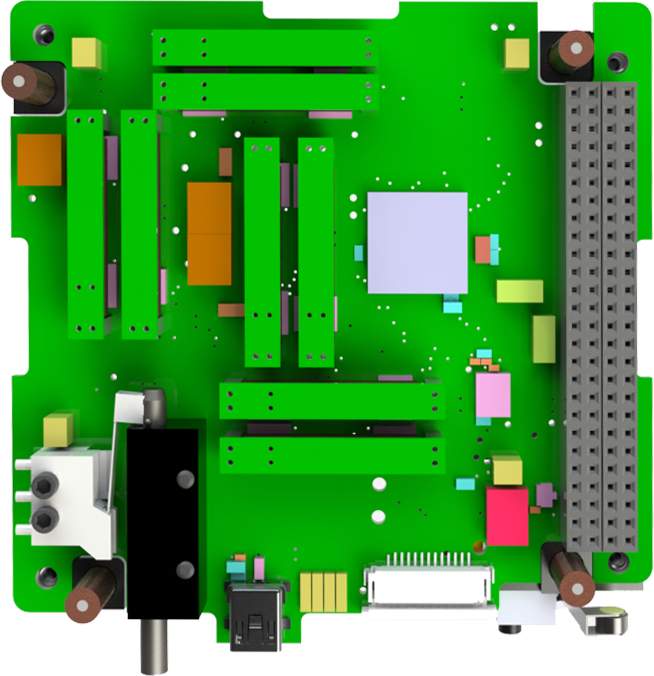
\includegraphics[width=\linewidth]{ACDS-board-render}};
            \begin{scope}[x={(image.south east)},y={(image.north west)}]
                \path (0.19,0.35) coordinate (PP)
                      %(0.30,0.27) coordinate (PP)
                      (0.39,0.09) coordinate (USB)
                      (0.45,0.70) coordinate (TqX1)
                      (0.36,0.70) coordinate (TqX2)
                      (0.18,0.70) coordinate (TqX3)
                      (0.25,0.70) coordinate (TqX4)
                      (0.45,0.895) coordinate (TqY1)
                      %(0.45,0.89) coordinate (TqY1)
                      (0.45,0.93) coordinate (TqY2)
                      (0.50,0.37) coordinate (TqY3)
                      (0.50,0.49) coordinate (TqY4)
                      (0.14,0.13) coordinate (TqZ1)
                      (0.05,0.87) coordinate (TqZ2)
                      (0.88,0.90) coordinate (TqZ3)
                      (0.89,0.15) coordinate (TqZ4)
                      (0.96,0.095) coordinate (SS);
              %draw axis
                %\path (0.15,0.72) coordinate (axOrig);
                %\draw[->,red,very thick] (axOrig) to +(-88.3:0.1) coordinate (X);
                %\node[red,below of=X] (Xl) {X};
                %\draw[->,magenta,very thick] (axOrig) to +(180.5:0.1) coordinate (Y);
                %\node[magenta,left of=Y] (Yl) {Y};
                %\draw[->,red,very thick] (axOrig) to +(-90:0.1) coordinate (Z);
                %\node[red,below of=Z] (Zl) {Z};
              \end{scope}
        \end{tikzpicture}
    \end{minipage}\begin{minipage}{0.30\linewidth}
        \begin{itemize}\setlength{\parskip}{0pt}
            %\item[\kern-0.2em] \tikz[na] \coordinate (TqXi); X torquers
            \item[\kern-0.2em] \tikz[na] \coordinate (TqYi); Y torquers
            \item[\kern-0.2em] \tikz[na] \coordinate (TqZi); Z torquers
            \item[\kern-0.2em] \tikz[na] \coordinate (SSi); Separation switch
            %\item[\kern-0.2em] \tikz[na] \coordinate (PPi); Pull Pin
            %\item[\kern-0.2em] \tikz[na] \coordinate (USBi); \acf{USB} connection
        \end{itemize}
    \end{minipage}

    \begin{tikzpicture}[overlay,remember picture]
            \path[->,blue,very thick] (PPi) edge (PP);
            \path[->,blue,very thick] (USBi) edge (USB);
            \path[->,red,very thick] (TqXi) edge (TqX1);
            %\path[->,red,very thick] (TqXi) edge (TqX2);
            \path[->,red,very thick] (TqXi) edge (TqX3);
            %\path[->,red,very thick] (TqXi) edge (TqX4);
            \path[->,black,very thick] (TqYi) edge (TqY1);
            %\path[->,black,very thick] (TqYi) edge (TqY2);
            \path[->,black,very thick] (TqYi) edge (TqY3);
            %\path[->,black,very thick] (TqYi) edge (TqY4);
            \path[->,magenta,very thick] (TqZi) edge (TqZ1);
            \path[->,magenta,very thick] (TqZi) edge (TqZ2);
            \path[->,magenta,very thick] (TqZi) edge (TqZ3);
            \path[->,magenta,very thick] (TqZi) edge (TqZ4);
            \path[->,blue,very thick] (SSi) edge (SS);
    \end{tikzpicture}
    \caption{The \ac{ARC} \ac{ACDS} board.}
    \label{fig:boardRender}
\end{figure}

In addition to the \ac{ACDS} hardware, the \ac{ACDS} board also contains the pull pin and \ac{USB} connection port. This is located on the \ac{ACDS} board because it is the only board that is accessible through the \ac{SPB}. The pull pin and \ac{USB} connection connect directly to the header and are not connected to the core \ac{ACDS} hardware. 

The Z-axis torquers are housed inside the standoffs which are located on the four corners of the board. The \ac{ACDS} board shape has been modified from the standard board shape to accommodate the torquers and standoffs. This is visible in \cref{fig:boardRender}. The notches are designed to fit the z-axis torquer standoffs and keep them aligned in the proper orientation. The torquers fit into a hole drilled into the standoffs and are held in place with epoxy. 

The standard board shape has also been modified to allow the \ac{USB} connector to be placed closer to the access port so that the \ac{USB} cable can be easily plugged in. This is also visible in \cref{fig:boardRender}.

\subsection{Bus Communication}

The subsystems of the \ac{ARC} will communicate with each other using the ARCBus. The ARCBus consists of shared connections between the subsystems to transmit commands and data. The ARCBus will primarily used by the \ac{ACDS} to get sensor data from the \ac{LEDL} and send and receive data to the ground station through the COMM system. Commands are transmited using an \ac{I2C} bus and large blocks of data are transfered using a \ac{SPI} bus which is negotiated using the \ac{I2C} bus.

\section{Components of the \acl{ACDS}}

\afterpage{\begin{landscape}
\begin{figure}[p]
    \centering
    % vim: filetype=tex spell 

% We need layers to draw the block diagram
\pgfdeclarelayer{background}
\pgfdeclarelayer{foreground}
\pgfdeclarelayer{Hardware}
\pgfdeclarelayer{CPU}

\pgfsetlayers{background,Hardware,CPU,main,foreground}

\begin{tikzpicture}
    %first draw ARCbus
    \begin{pgfonlayer}{Hardware}
        \node[draw=black,minimum height=10cm,minimum width=1cm] (arcbus) at (0,0) {\rotatebox{90}{\acs{ARC} Bus}};
    \end{pgfonlayer}

    \begin{scope}[start chain]
        \node[perif,node distance=1.5cm,right=of arcbus]    (SPI_IIC)  {\rotatebox{90}{\acs{SPI} + \acs{I2C}}};
        \node[prog]    (command) at ([yshift=15mm,xshift=3mm]SPI_IIC) {command and control};

        \begin{scope}[start branch=storage going below]
            \node[point,node distance=15mm,on chain] (nexus) {};
            \node[prog,text width=7em,node distance=5mm,on chain=going right]       (housek)   {Housekeeping};
            \node[perif,node distance=2mm]    (SPI)      {\acs{SPI}};
            \node[hardware]    (SD)       {\acs{SD}};
        \end{scope}

        \node[prog]    (lpmt)     {\acs{LPMT} algorithm};
        \node[perif,join=by dataL]       (tqio)    {\rotatebox{90}{\acs{GPIO}}};
        \node[hardware,join=by dataL]    (hbridge)    {H-Bridges};

        \begin{scope}[start branch=power going left]
            \node [power,on chain=going above]   (cap) {Capacitors (one per axis)};
            \node [power]      (capchg) {Capacitor charging circuit};
        \end{scope}

        \node[hardware,on chain=going below]    (torquers)    {Torquers};

    \end{scope}

    \begin{scope}[start chain=LEDL going below]
        \node[hardware,node distance =2cm,left=of arcbus]  (LEDL)  {\acs{LEDL} \textmu{}C};
        \begin{scope}[start branch=gyro going above]
            \node[hardware,node distance=5mm]   (gyro) {Gyros};
        \end{scope}
        \node[hardware,text width=8em]   (mag) at ([yshift=-1.5cm]LEDL)     {Magnetometer};
    \end{scope}

    %draw CPU box
    \begin{pgfonlayer}{CPU}
        \node (push) at ([yshift=1.3cm]command) {};
        \node[CPU,fit=(SPI_IIC) (command) (lpmt) (housek) (SPI) (tqio) (push)] (cpu) {};
        \node[above,anchor=south west] at (cpu.north west) {\acs{ACDS} \textmu{}C};
    \end{pgfonlayer}

    %draw board boxes
    \begin{pgfonlayer}{Hardware}
        %draw LEDL board
        \node[PCB,fit=(LEDL) (gyro)] (LEDLpcb) {};
        \node[above,anchor=south west] at (LEDLpcb.north west) {\acs{LEDL}};
        %draw SPB
        \node[PCB,fit=(mag)] (spb) {};
        \node[above,anchor=south west] at (spb.north west) {\acs{SPB}};
        %draw ACDS
        \node[PCB,fit=(cpu) (SD) (hbridge) (cap) (capchg) (torquers)] (ACDSpcb) {};
        \node[above,anchor=south west] at (ACDSpcb.north west) {\acs{ACDS}};
    \end{pgfonlayer}

    \begin{pgfonlayer}{foreground}
        \node[draw=black,fill=white] (legend) at (ACDSpcb.south east) {\begin{tikzpicture}
            \begin{scope}[start chain=going below,node distance=1mm]
                \node[power,text width=6em] (cleg) {Power Component};
                \node[prog,text width=6em] {Program Component};
                \node[perif,text width=6em] {Peripheral};
                \node[hardware,text width=6em,minimum height=1em] {Hardware};
            \end{scope}
            \begin{scope}[start chain=going below,node distance=0cm,text width=6em]
                \node[on chain,left=of cleg] {};

                \node[on chain,rectangle] (pl) {Power Line};
                \path[powerL] (pl.west) ++(-5mm,0) -- ++(-1cm,0);

                \node[on chain,rectangle] (dl) {Data Line};
                \path[dataL] (dl.west) ++(-5mm,0) -- ++(-1cm,0);

                \node[on chain,rectangle] (bl) {Bus Line};
                \path[Bus] (bl.west) ++(-5mm,0) -- ++(-1cm,0);
            \end{scope}
            
        \end{tikzpicture}};
        \node[anchor=north west] at (legend.north west) {\large \bf Legend};
    \end{pgfonlayer}

    \path[Bus] (LEDL) -- (arcbus);
    \path[Bus] (SPI_IIC) -- (arcbus);
    \path[Bus] (LEDL) -- (mag);
    \path[dataL] (LEDL) -- (gyro);

    %dummy nodes for getting good connections
    \node[point] (shift1) at ([yshift=8mm]housek) {};
    \node[point] (shift2) at ([xshift=-8mm]nexus) {};

    \path[dataL] (SPI_IIC.north) |- (command.west);
    \path[dataL] (SPI_IIC) -| (shift2);
    \path[dataL] (nexus) -- (housek);
    \path[dataL] (lpmt.south) |- (shift1);
    \path[dataL] (command.south) |- (shift1);
    \path[dataL] (shift1) -- (housek);
    \path[dataL] (shift2) -- (housek);
    \path[dataL] (command) -- (lpmt);
    \path[dataL] (housek) -- (SPI);
    \path[dataL] (SPI) -- (SD);

    \path[powerL] (capchg) -- (cap);
    \path[powerL] (cap) -- (hbridge);
    \path[powerL] (hbridge) -- (torquers);

\end{tikzpicture}



    \caption{Block Diagram of the CubeSat \acs{ACDS} system}
    \label{fig:ACDS-block2}
\end{figure}
\end{landscape}}

The block diagram for the CubeSat hardware used to implement the \ac{ACDS} is shown in \cref{fig:ACDS-block}. The hardware necessary for the \ac{ACDS} is spread over multiple subsystems of the \ac{ARC}. The \ac{ACDS} board contains the torquers, driving hardware along with the microcontroller which will run the attitude control algorithm. There is one two-axis magnetometer located on each of the six of the \acp{SPB}. These are used by the \ac{ACDS} to calculate rotation rates and calculate the magnetic dipole moment required to generate the necessary torque. Spreading the magnetometers across all six faces should give some degree of noise immunity and redundancy. The \ac{LEDL} board also contains \ac{MEMS} angular rate sensors as a redundant measurement of the rotation rate of the \ac{ARC}. The sensors on the \acp{SPB} are read by the \ac{LEDL}, which then forwards the magnetometer and angular rate measurements to the \ac{ACDS}.

\section{Torquers}

\Cref{fig:torquers} illustrates the torquer locations within the \ac{ARC}. The torquers consist of a hard magnetic core surrounded with a coil of wire. There are a total of twelve torquers on the \ac{ARC}, with four in each axis. The torquers are flipped using a driving circuit that causes a current pulse to flow through the coil. The driving hardware for the torquers is designed to flip one torquer in each axis every second.

\begin{figure}[!ht]
    \centering
    \begin{minipage}{0.25\linewidth}
        \begin{itemize}\setlength{\parskip}{0pt}
            \item[\kern-0.2em] Magnetometer \tikz[na] \coordinate (MAGi);
            \item[\kern-0.2em] Y torquers \tikz[na] \coordinate (YTi);
            \item[\kern-0.2em] X torquers \tikz[na] \coordinate (XTi);
            \item[\kern-0.2em] Z torquers\tikz[na] \coordinate (ZTi);
        \end{itemize}
    \end{minipage}\begin{minipage}{0.55\linewidth}
        \begin{tikzpicture}[remember picture] 
            \node[anchor=south west,inner sep=0] (image) at (0,0) {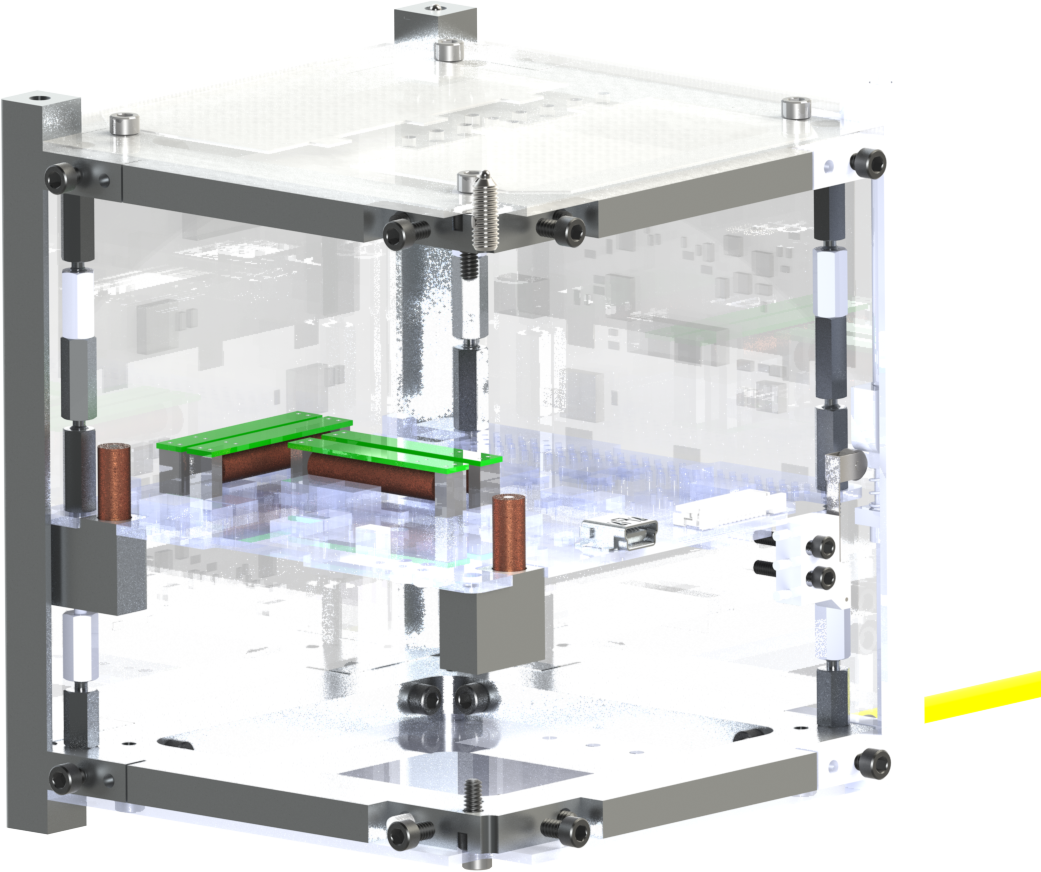
\includegraphics[width=\linewidth]{torquers}};
            \begin{scope}[x={(image.south east)},y={(image.north west)}]
                \fill[blue,fill opacity=0.3] (0.722,0.712) -- (0.74,0.709) -- (0.74,0.683) -- (0.723,0.685) -- cycle;
                \path (0.722, 0.7) coordinate (MAG)
                      (0.28,0.49) coordinate (XT)
                      (0.208,0.51) coordinate (YT)
                      (0.1,0.45) coordinate (ZT1)
                      (0.48,0.4) coordinate (ZT2);
              \end{scope}
        \end{tikzpicture}
    \end{minipage}

    \begin{tikzpicture}[overlay,remember picture]
            \path[->,red,very thick] (MAGi) edge (MAG);
            \path[->,red,very thick] (XTi) edge (XT);
            \path[->,red,very thick] (YTi) edge (YT);
            \path[->,red,very thick] (ZTi) edge (ZT1);
            \path[->,red,very thick] (ZTi) edge (ZT2);
    \end{tikzpicture}
    
    \caption{Torquer locations within the \ac{ARC}}
    \label{fig:torquers}
\end{figure}

\begin{figure}[!ht]
    \centering
    \begin{minipage}{1.7em}
        \setlength{\parskip}{2mm}
        Z2 \tikz[na] \coordinate (Z2i);

        X1 \tikz[na] \coordinate (X1i);

        X2 \tikz[na] \coordinate (X2i);

        X3 \tikz[na] \coordinate (X3i);

        X4 \tikz[na] \coordinate (X4i);

        Z1 \tikz[na] \coordinate (Z1i);
    \end{minipage}\hspace{2em}\begin{minipage}{0.35\linewidth}
        \centering
        \begin{tikzpicture}[remember picture] 
            \node[anchor=south west,inner sep=0] (image) at (0,0) {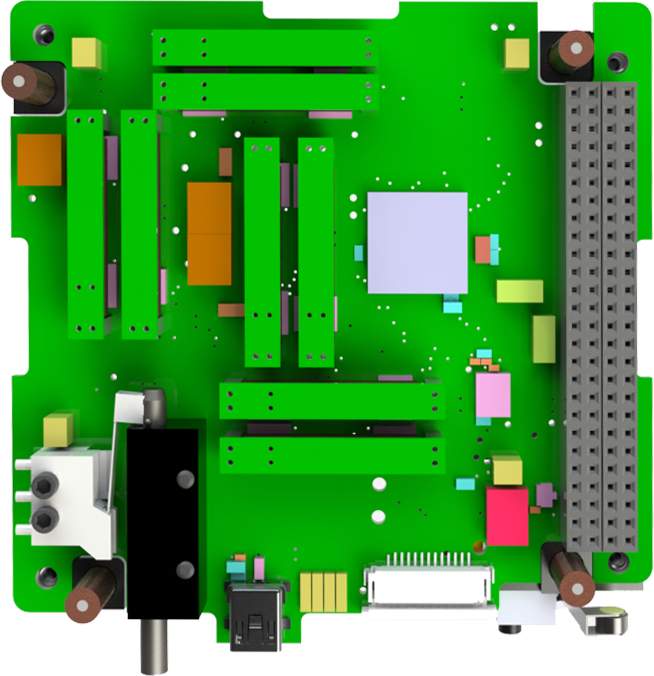
\includegraphics[width=\linewidth]{ACDS-board-render}};
            \begin{scope}[x={(image.south east)},y={(image.north west)}]
                \path 
                      (0.49,0.70) coordinate (X1)
                      (0.40,0.64) coordinate (X2)
                      (0.16,0.58) coordinate (X3)
                      (0.23,0.53) coordinate (X4)
                      (0.45,0.88) coordinate (Y1)
                      (0.45,0.93) coordinate (Y2)
                      (0.50,0.41) coordinate (Y3)
                      (0.50,0.33) coordinate (Y4)
                      (0.13,0.12) coordinate (Z1)
                      (0.04,0.87) coordinate (Z2)
                      (0.88,0.91) coordinate (Z3)
                      (0.89,0.14) coordinate (Z4);
              %draw axis
                %\path (0.15,0.72) coordinate (axOrig);
                %\draw[->,red,very thick] (axOrig) to +(-88.3:0.1) coordinate (X);
                %\node[red,below of=X] (Xl) {X};
                %\draw[->,magenta,very thick] (axOrig) to +(180.5:0.1) coordinate (Y);
                %\node[magenta,left of=Y] (Yl) {Y};
                %\draw[->,red,very thick] (axOrig) to +(-90:0.1) coordinate (Z);
                %\node[red,below of=Z] (Zl) {Z};
              \end{scope}
        \end{tikzpicture}
    \end{minipage}\hspace{2em}\begin{minipage}{1.7em}
        \setlength{\parskip}{2mm}
        \tikz[na] \coordinate (Z3i); Z3

        \tikz[na] \coordinate (Y2i); Y2

        \tikz[na] \coordinate (Y1i); Y1

        \tikz[na] \coordinate (Y3i); Y3

        \tikz[na] \coordinate (Y4i); Y4

        \tikz[na] \coordinate (Z4i); Z4
    \end{minipage}

    \begin{tikzpicture}[overlay,remember picture]
            \path[->,blue,very thick] (X1i) edge (X1);
            \path[->,blue,very thick] (X2i) edge (X2);
            \path[->,blue,very thick] (X3i) edge (X3);
            \path[->,blue,very thick] (X4i) edge (X4);

            \path[->,black,very thick] (Y1i) edge (Y1);
            \path[->,black,very thick] (Y2i) edge (Y2);
            \path[->,black,very thick] (Y3i) edge (Y3);
            \path[->,black,very thick] (Y4i) edge (Y4);

            \path[->,magenta,very thick] (Z1i) edge (Z1);
            \path[->,magenta,very thick] (Z2i) edge (Z2);
            \path[->,magenta,very thick] (Z3i) edge (Z3);
            \path[->,magenta,very thick] (Z4i) edge (Z4);
    \end{tikzpicture}
    \caption{The \ac{ARC} \ac{ACDS} torquer locations.}
    \label{fig:TQloc}
\end{figure}
\subsection{Cores}

Most magnetic torquers use either an air core or a soft magnetic core. Ideally both an air or a soft core only produce torque while a current is running through the coil. A soft core will produce more torque for the same geometry and current compared to an air core. However, soft magnetic materials have some hysteresis that will continue to produce undesired torque after current stops flowing. Hard magnetic materials are chosen to have a large amount of hysteresis so that torque is still produced after the current stops flowing in the coil.

The torquer cores for the \ac{ARC} are made of Alnico1, which is a hard magnetic material. Core materials are chosen for their residual induction ($B_r$) and their coercive force ($H_c$). The torque produced for a given torquer geometry is proportional to $B_r$. This means that $B_r$ dictates the range of torques that are feasible. If $B_r$ is too small, then the torquers will have to be too big to fit in the satellite. If $B_r$ is too large, then it may not be possible to manufacture torquers that are small enough to give the desired torque. The current required to flip the torquer for a given coil and core geometry is determined by $H_c$. It is desirable to have a low $H_c$ so less energy is used for each flip. However, if $H_c$ is too low then the torquer can be flipped inadvertently.

\subsubsection{Core Sizing}

The torquer cores proposed \cite{Mentch11} consisted of a large and a small pair in each axis. The large pair were to be made of Alnico1 and produce a magnetic dipole moment of $0.022 \unit{A \cdot m^2}$. The small pair was proposed to have an inert core with a thin permalloy coating to give it a dipole moment of $0.00011 \unit{A \cdot m^2}$. All torquer cores were to be the same size, one inch long of $\sfrac{1}{16}$-inch diameter rod.

As discussed in \cite{Mentch11} the large cores were sized by first determining the desired torque for each torquer to produce then calculating the necessary dipole moment. Simulation was used to refine the required dipole moment. Alnico5 was the core material that had been used in previous experiments for much larger cores\cite{Mentch11}\todo{Look for other reference?}. The minimum manufactured size of alnico rods is $\sfrac{1}{16}$-inch. It is desirable to have a length to diameter ratio greater than 10, which fixes the minimum torque that can be achieved. The torque using Alnico5 was larger than the desired torque so Alnico1 was used instead, which has a lower residual induction. 

The proposed size of the small torquers was $\sfrac{1}{200}$th the torque of the alnico torquers. The fabrication of the proposed torquer was not completed and even if it had it is not clear that testing could have been done to quantify the dipole moment. In addition to fabrication and testing issues there is the problem of balancing the alnico cores. Because of theses difficulties the original design for the small torquers was dropped and an extra set of Alnico torquers was added in their place. The charge time was also shortened from 10 seconds to 1 second.

\begin{comment}
\subsubsection{Measuring Dipole Moment}

Determining the dipole moment is not an easy task as the dipole moments are quite small. \future{I should probably do some dipole measurements and write it up.}
\end{comment}

\subsection{Coils}

The coils used to drive the torquers are made from 248 turns of 26~AWG wire in four layers. The current spike to flip the torquer peaks around 7~A which is significantly higher than 26~AWG can handle with continuous current. However, because the pulse duration is short it is not a problem.

A 1~inch long solenoid with 7~A through 248 turns of wire has a coercive force of 68~kA/m. This is significantly higher than the coercive force of alnico1 which is 37~kA/m\cite{AlnicoProp}. This shows that the solenoids on the \ac{ARC} are more than capable of flipping a torquer.

\subsection{Drivers}

\begin{figure}[htb!]
    \centering
    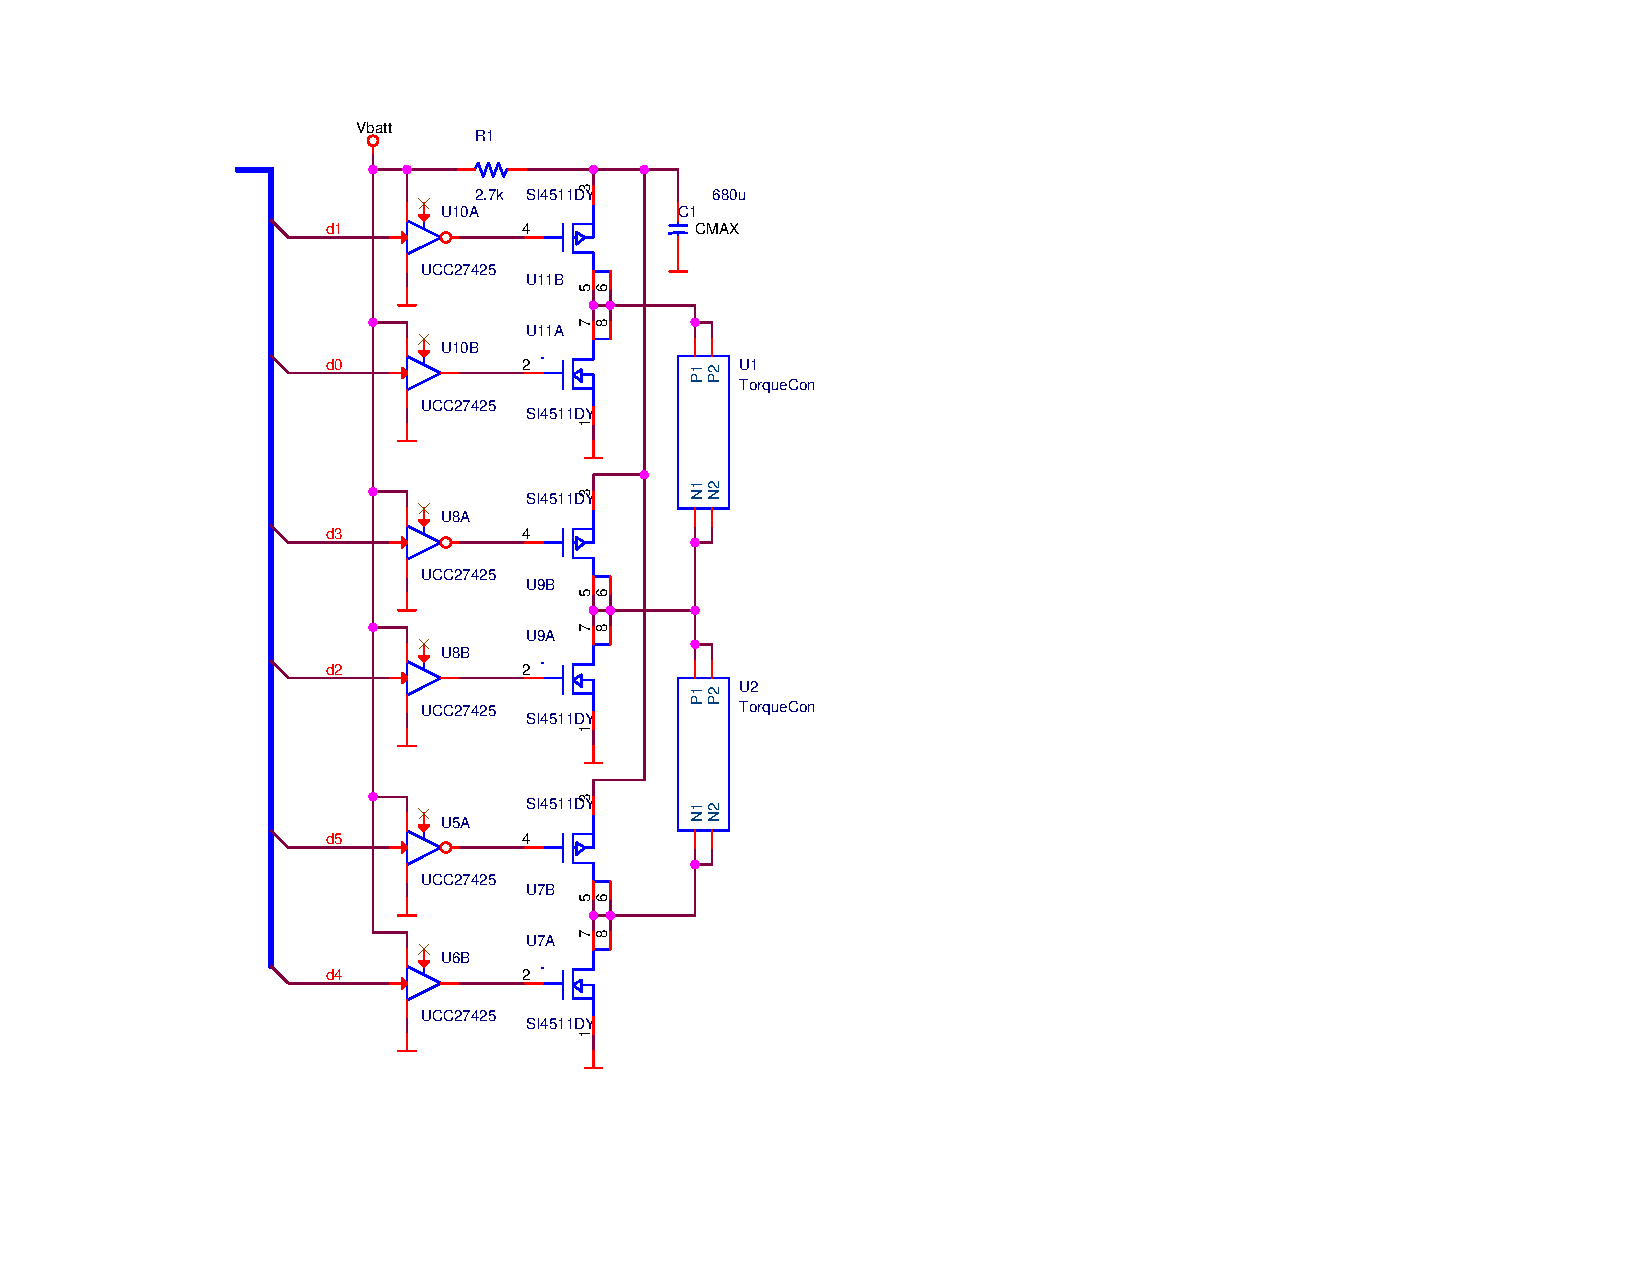
\includegraphics[height=0.5\textheight]{Figures/driverSchematic}
    \caption{Torquer Driver schematic}
    \label{fig:drive}
\end{figure}

The schematic of the circuit used to drive a pair of torquers is shown in \cref{fig:drive}. Each pair of torquers is driven by three complimentary pairs of \acp{MOSFET}.  The \acp{MOSFET} are driven by three pairs of \ac{MOSFET} drivers that are controlled by the \ac{ACDS} microcontroller. The capacitor C1 is shared between both pairs of torquers in each axis giving a total of three capacitors on the \ac{ACDS} board. This means that only one torquer in each axis can be flipped each second. 

In the idle state, all of the \acp{MOSFET} are off and the torquer coils are floating. This prevents unwanted currents from flowing in the torquers. If \acp{MOSFET} are left on, providing a current path between the coil terminals, currents can be induced in the coils as the satellite turns and the magnetic field in the torquers changes. To flip a torquer, one end of the torquer is shorted to ground using one of the N-Channel \acp{MOSFET} and the other end is shorted to capacitor C1 using one of the P-Channel \acp{MOSFET}. After a 2 ms delay, the \acp{MOSFET} are switched off and C1 begins to recharge.

\subsubsection{Driving Waveform}

\begin{figure}[htb!]
    \centering
    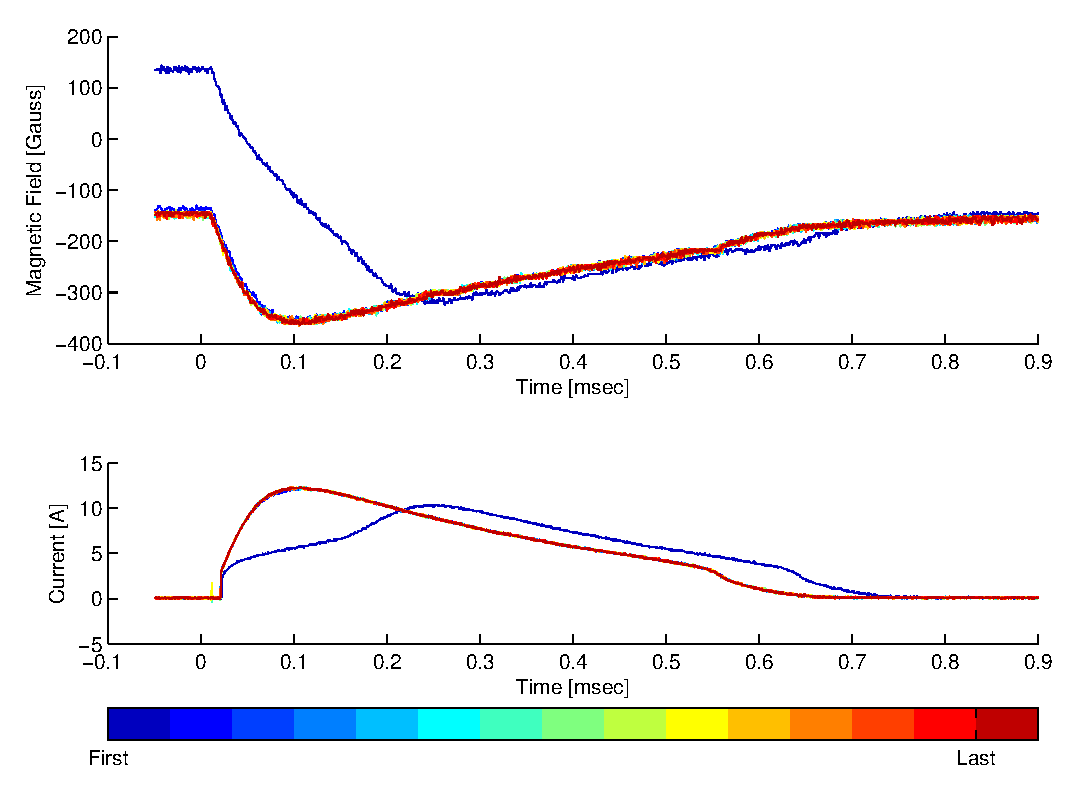
\includegraphics[width=\textwidth]{torquer-waveforms}
    \caption{Torquer driving waveform showing multiple torquer flips.}
    \label{fig:driveWV}
\end{figure}

\Cref{fig:driveWV} shows the driving waveform when driving a torquer multiple times in the same direction. The first torquer flip is shown in blue and the last flip is shown in red. The first waveform is the only waveform that differs significantly from the subsequent waveforms because the torquer is fully saturated in the first flip, thus demonstrating that the driving circuit is adequate to completely flip the torquers using a single 1~ms pulse.

The magnetic field waveform for the fist flip starts at about +125~Gauss. This is because the torquer was flipped in the opposite direction before the test started. The reset of the waveforms start at about -125~Gauss. This is because the first flip drives the torquer into saturation flipping the torquers direction of magnetization. For all of the flips after the first flip, the change in magnetic field waveform is only due to the torquer coil and not to an actual torquer flip.

The current waveforms also show changes due to torquer saturation. For the first flip the current initially increases at a slower rate. This is because, on the Alnico1 B-H curve, the slope is steeper closer to the B-axis resulting in a higher inductance. As the torquer reaches saturation, the inductance of the torquer goes down and the rate of change of current increases. For the subsequent torquer flips, the torquer is already saturated so the inductance is low and the driving current reaches its peak much faster.

\begin{figure}[htb!]
    \centering
    \begin{tikzpicture}[remember picture,node distance=1em]
        \def\sysx{0.8}
        \begin{pgfonlayer}{background}
            \node[anchor=south west,inner sep=0] (image) at (0,0) {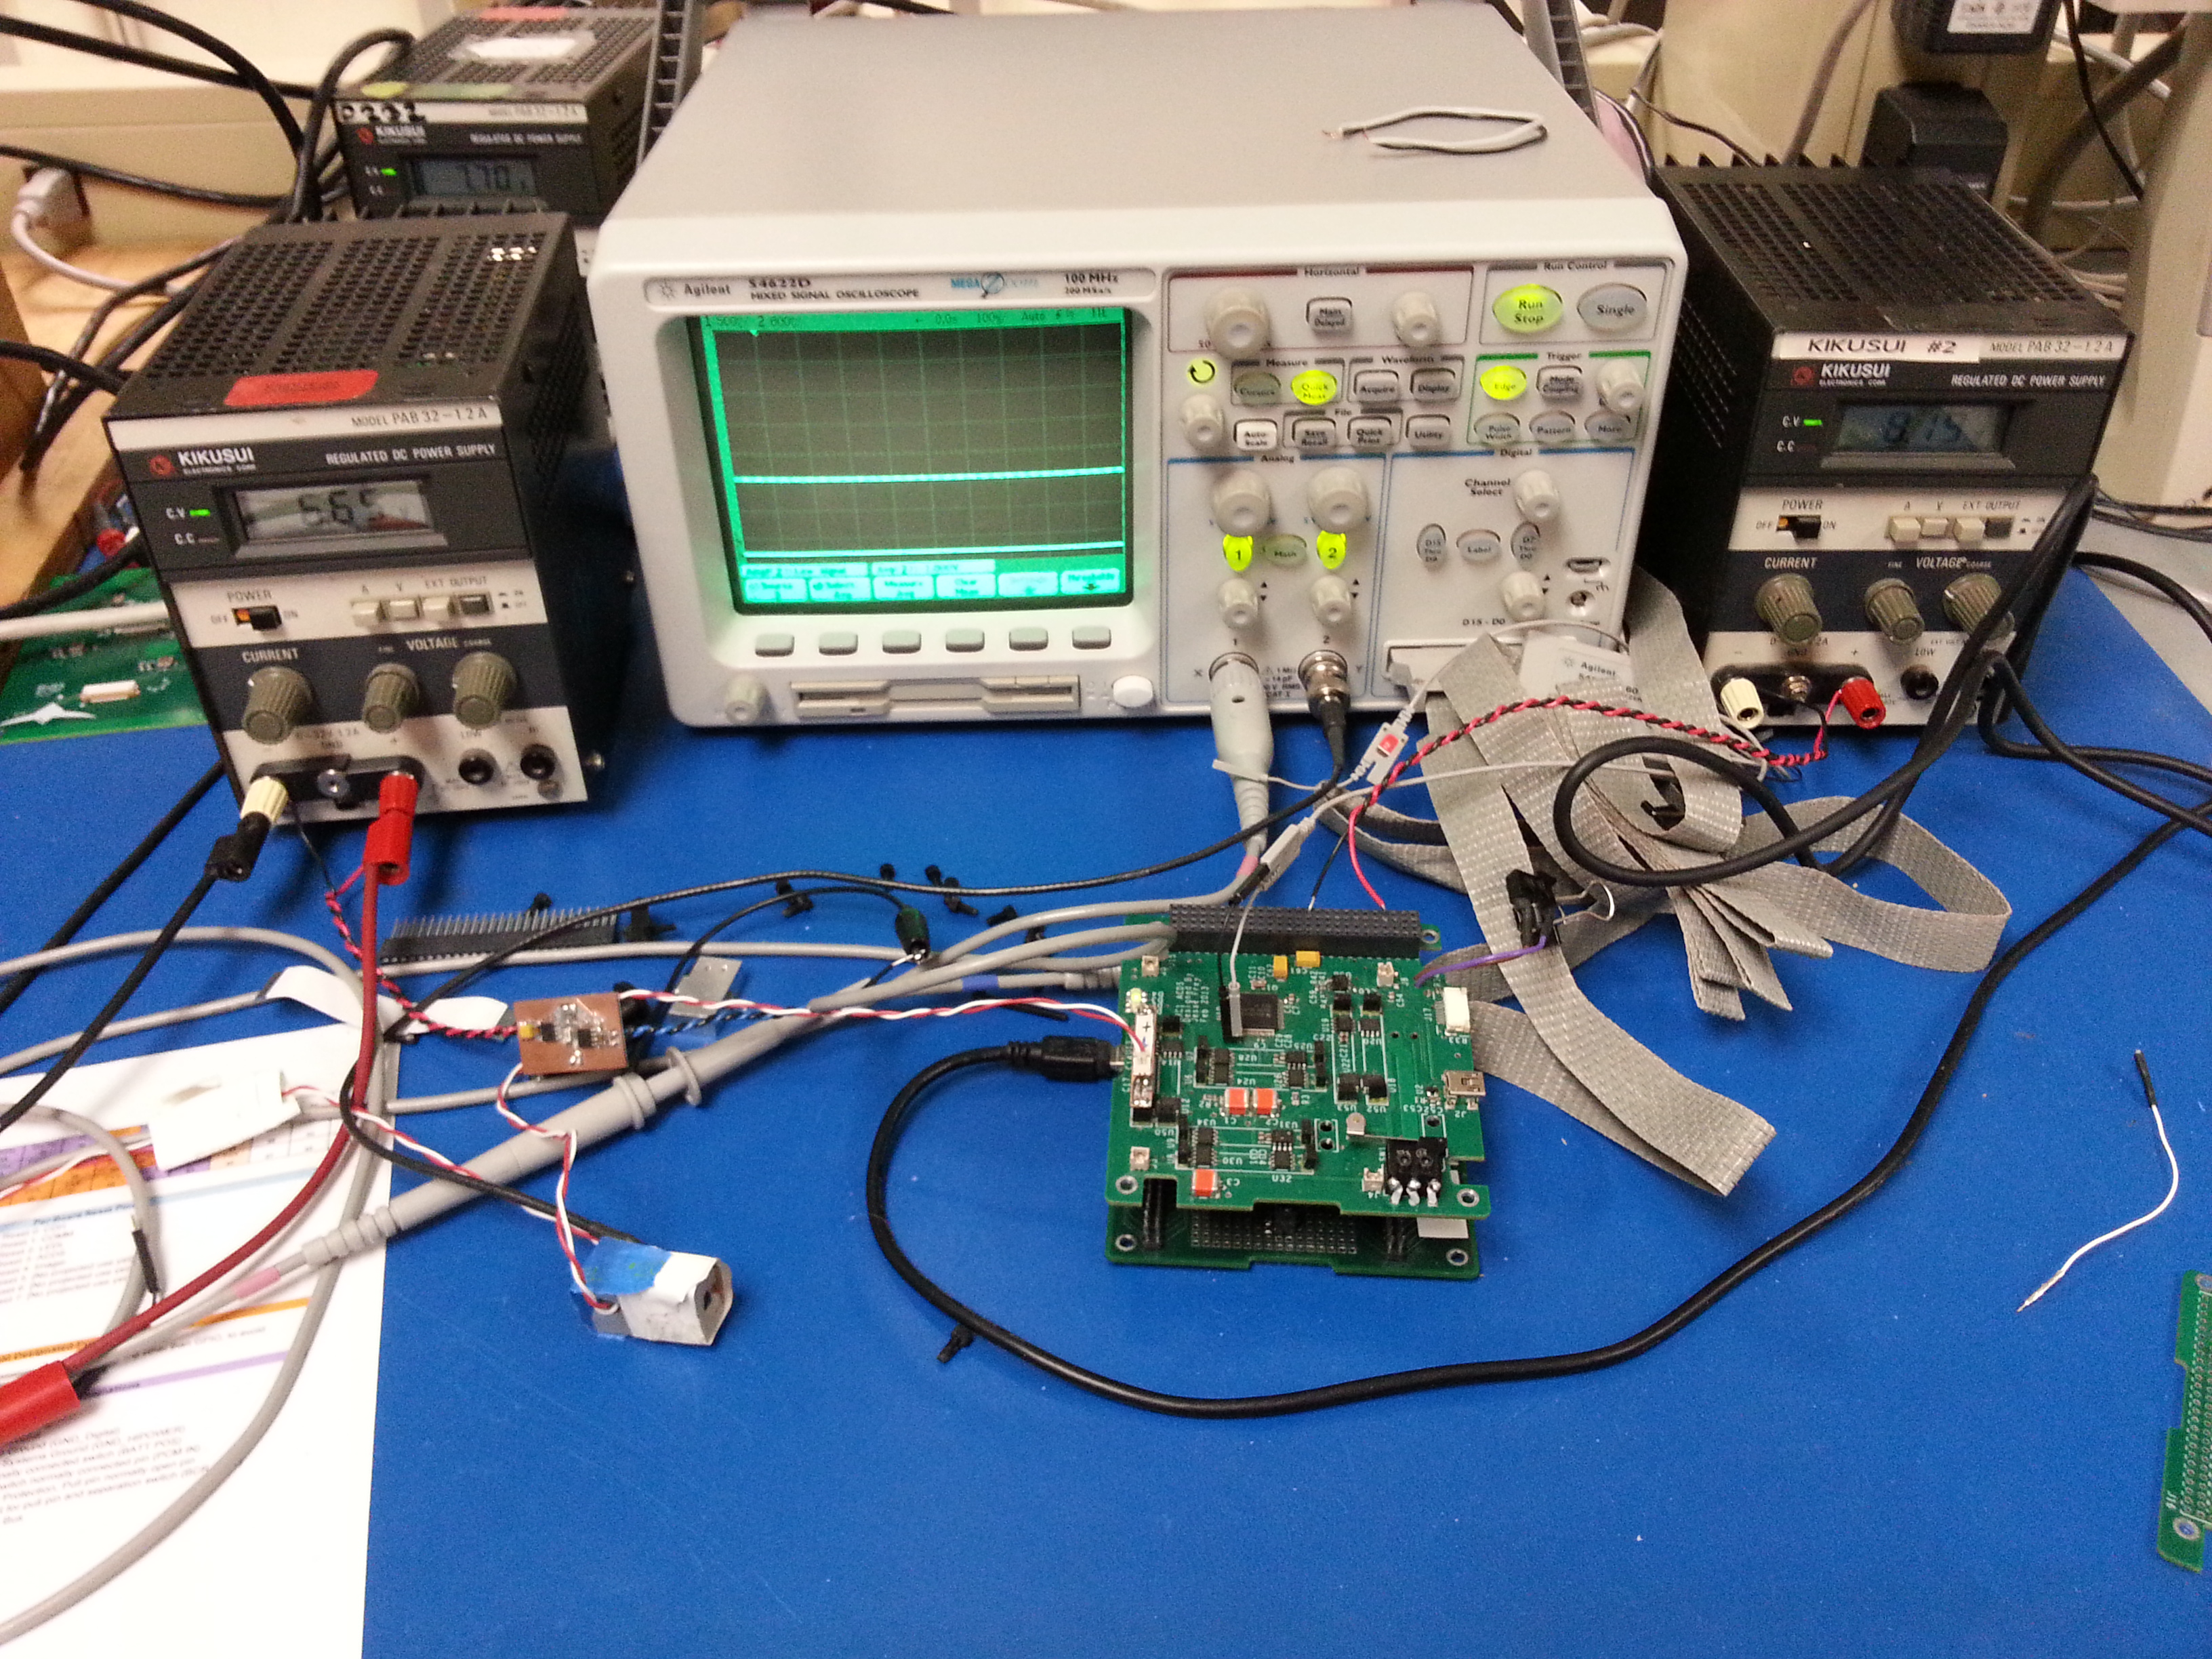
\includegraphics[width=\linewidth]{torquer-waveform-setup}};
        \end{pgfonlayer}
        %insert detail image
        \begin{scope}[x={(image.south east)},y={(image.north west)}]
            \node[inner sep=0] (detail) at (0.13,0.19) {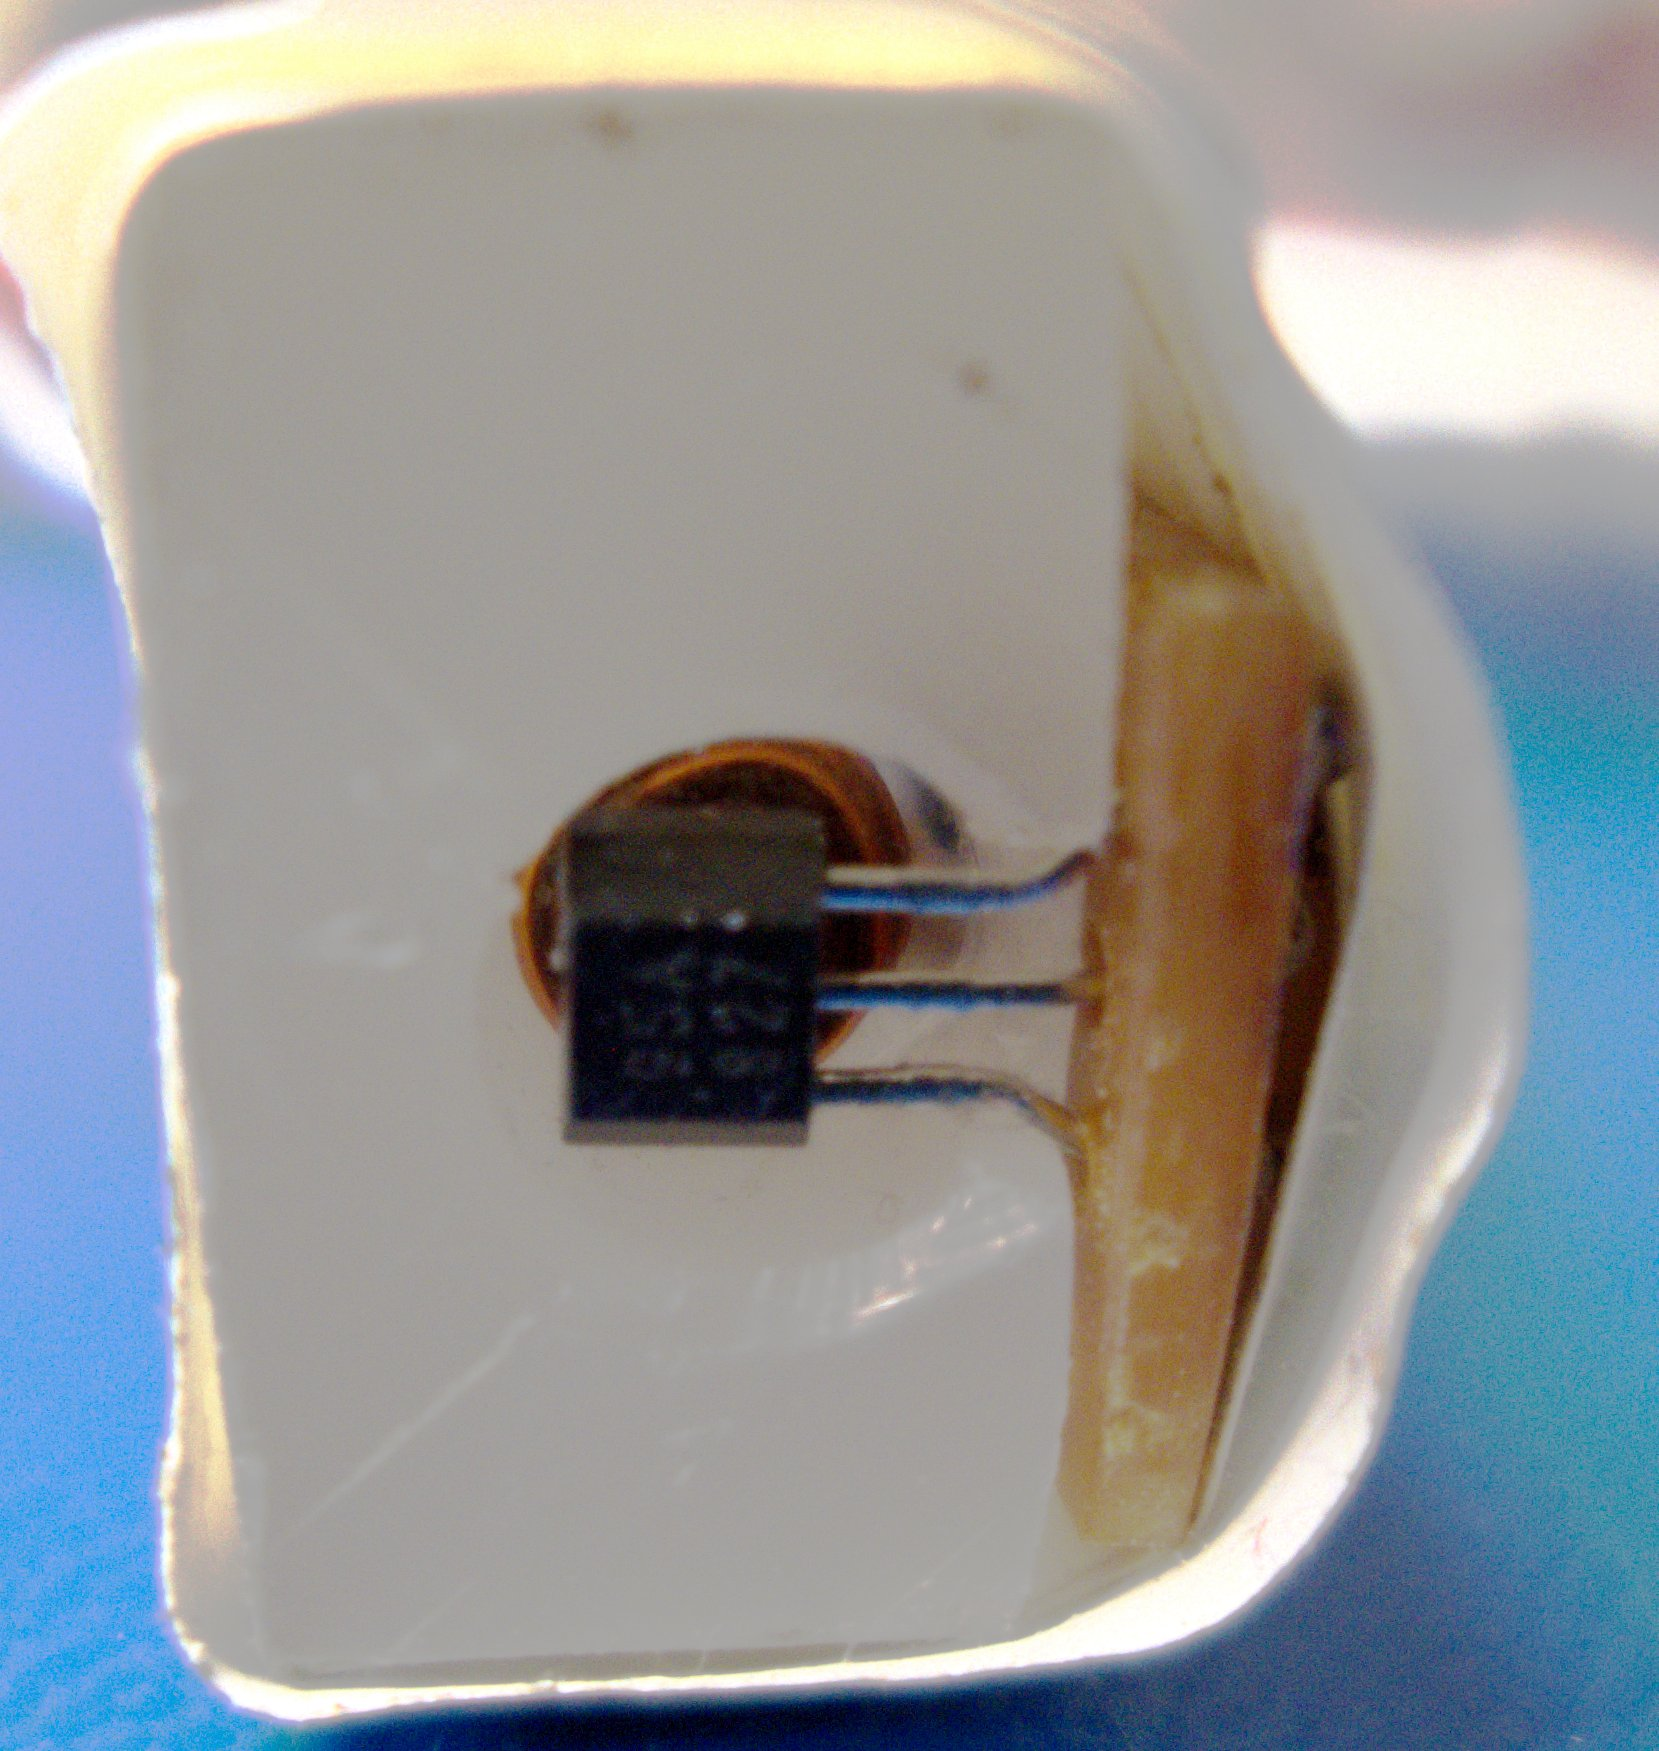
\includegraphics[width=1in,angle=-90]{testing-sensor}};
            %declare coordinates for box around sensor
            \path   (0.31,0.17) coordinate (box1)
                    (0.31,0.22) coordinate (box2)
                    (0.28,0.22) coordinate (box3)
                    (0.28,0.17) coordinate (box4);
            %draw box around sensor detail
            \draw[magenta,very thick] (detail.south east) -- (detail.south west) -- (detail.north west) -- (detail.north east) -- cycle;
            %draw box around sensor
            \draw[red,very thick] (box1) -- (box2) -- (box3) -- (box4) -- cycle;
            %draw ``expanding lines'' to detail
            \begin{pgfonlayer}{background}
                \draw[red,very thick] (box1) -- (detail.south east);
                \draw[red,very thick] (box2) -- (detail.north east);
                \draw[red,very thick] (box3) -- (detail.north west);
                \draw[red,very thick] (box4) -- (detail.south west);
            \end{pgfonlayer}
        \end{scope}
    \end{tikzpicture}
    \caption{Setup for measuring \cref{fig:driveWV,fig:satWV}. The Hall effect sensor on the end of the torquer is shown in detail.}
    \label{fig:WVsetup}
\end{figure}

\Cref{fig:WVsetup} shows the hardware used to take the data for \cref{fig:driveWV,fig:satWV}. The \ac{ACDS} board was used to drive the torquers. To communicate with the \ac{ACDS}, another microcontroller board was used along with a \ac{USB}-to-serial converter. The torquer connects to the \ac{ACDS} board through a current sensor which is read by the oscilloscope. The torquer is placed inside a plastic housing with an attached Hall effect sensor. The hall effect sensor is located against the end of the torquer and is read by the oscilloscope. A pin on the \ac{ACDS} microcontroller is  used to trigger the scope which is automatically configured by a \matlab script that communicates with the \ac{ACDS} board and the oscilloscope.

\begin{figure}[htb!]
    \centering
    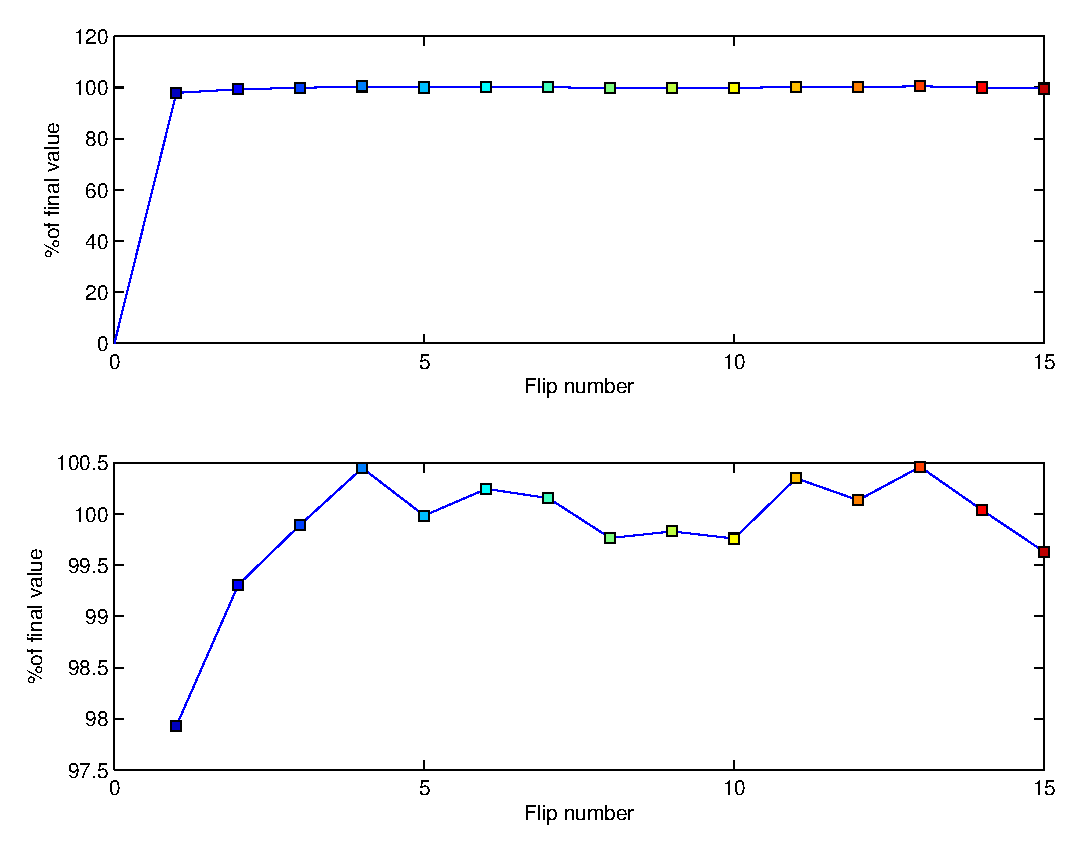
\includegraphics[width=\textwidth]{torquer-multiflip}
    \caption{Torquer saturation}
    \label{fig:satWV}
\end{figure}

The measured field that the Hall effect sensor reads is highly dependant on the distance from the torquer. Using the residual induction of Alnico1, 7200 Gauss from \cite{AlnicoProp} and the calculator from \cite{DexterField} the calculated magnetic field from the torquers is 155~Gauss at 0.05~in from the face of the torquer. This is close to what is shown in \cref{fig:driveWV}. As the distance from the face increases to 0.1,~0.2~and~0.3~in the field decreases to 46,~12~and~5~Gauss, respectively.

\Cref{fig:satWV} shows how the torquer field changes as the number of flips increases. Both graphs show the same data, with the lower graph zoomed in to better show the points after the first flip. The 0\% point is found by averaging 20 samples from the beginning of the first magnetic field waveform in \cref{fig:driveWV}. The rest of the points are found by averaging the last 20 samples of the magnetic field waveforms from \cref{fig:driveWV}. The first flip gets the torquer field to within 97\% of the final value and after two flips it has reached the final value. 

\subsection{Torquer Diagnostics}

\begin{figure}[htb!]
    \centering
    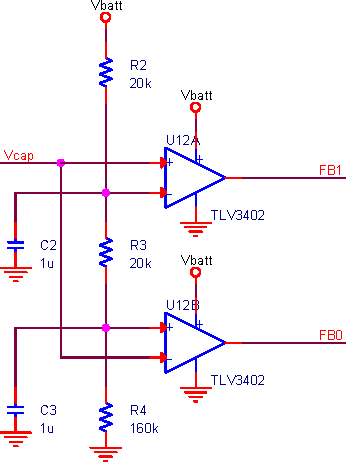
\includegraphics{fb-comp}
    \caption{Torquer feedback comparators}
    \label{fig:fb-comp}
\end{figure}

\Cref{fig:fb-comp} shows the torquer feedback comparators that are used to detect if the torquers and drivers are functioning properly in flight. Vcap is the voltage from capacitor C1 in \cref{fig:drive}. The comparator outputs, FB0 and FB1, have open drain outputs that are pulled up to logic hi by internal resistors on the MSP430 inputs. U12A  is used to determine if the capacitor is charged and U12B is used to detect if the capacitor is discharged. The comparators are checked both before and after a torquer flip to see if the capacitor was charged before an attempted flip and discharged after. If the capacitor did not discharge, then the torquer did not flip, probably because of a bad connection somewhere. This information is logged in flight and can be downlinked to analyze if the torquers are firing correctly.

\todo[inline]{Need some discussion of what is done with the info but also need to figure out what should be done.}


\section{Sensors}

The only sensor specified in \cite{Mentch11} was a magnetometer. The magnetometer was proposed to be used to determine the angular rates of the \ac{ARC} as well as part of the torque equation. Because the torque produced by the torquers depends on the Earth's magnetic field, the Earth's magnetic field must be known in order for the algorithm to compute the necessary dipole moment. The accuracy of the magnetometer was not specified but it needs to be able to determine rotation rates accurately enough for the \ac{ACDS} to work.

\subsection{Magnetometer}

The magnetometers on the satellite are Honeywell HMC1052 \ac{AMR} sensors. These sensors use \ac{AMR} elements in a bridge configuration to measure the field in each axis. The HMC1052 is a 2-axis sensor that measures the field in the axis that are parallel to the board that it is mounted on (X and Y). Each face of \ac{ARC} will have a single HMC1052 giving a total of 4 measurements in each axis.

The magnetometers are located on the back of the \acs{SPB}, shown in \cref{fig:SPB}. The magnetometer, with surrounding circuitry, is visible on the back of the board as are the \ac{ADC} and amplifier. An accelerometer is also located on the back of the solar panel board and is used for a different mission objective. The data connector powers the sensors and provides access to the sensor data.

\subsubsection{Magnetometer Amplifier}

The \ac{SPB} also contains an amplifier to amplify the magnetometer signal before it is read by the \ac{ADC}. This allows the output voltage of the magnetometer to fill the input range of the \ac{ADC}. The required range of the magnetometer will be largely dependent on the torquer geometry and could be more then the \textpm 600~mGauss or so of Earth's field. The amplifier can be used to trade range for resolution depending on what is needed.

\begin{equation}
    \label{eq:amp-gain}
    A = \frac{V_{adc}}{B_{max} \cdot V_{bridge} \cdot S_s + V_{os} \cdot V_{bridge}}
\end{equation}

\Cref{eq:amp-gain} shows the equation used to calculate the amplifier gain. The maximum voltage readable by the \ac{ADC}, $V_{adc}$, is divided by the maximum expected output from the magnetometer. The maximum output from the magnetometer is found by adding the output due to the desired full scale field and the maximum possible bridge offset.

%The gain for the amplifier can be calculated as follows: If the maximum output range of the sensor is restricted to \textpm 4 Gauss. With a bridge voltage of 3.3 V and a sensitivity of 1~mV/V/Gauss, this results in a \textpm 13.2~mV voltage swing. The bridge offset is \textpm 1.25~mV/V or \textpm 4.125~mV. This results in a total possible swing of \textpm 17.325~mV. The input voltage range of the \ac{ADC} is \textpm 1.65~V. This results in a gain of about 95. 

\begin{equation}
    \label{eq:amp-gain-calc}
    \begin{split}
        A &= \frac{1.65~\unit{V}}{4~\unit{Gauss} \cdot 3.3~\unit{V} \cdot 1~\unit{mV/V/Gauss} + 1.25~\unit{mV/V} \cdot 3.3~\unit{V}}\\ 
          &= \frac{1.65~\unit{V}}{13.2~\unit{mV} + 4.125~\unit{mV}} \\
          &= \frac{1.65~\unit{V}}{17.325~\unit{mV}} \\
          &= 95.24
    \end{split}
\end{equation}

\Cref{eq:amp-gain-calc} shows the gain calculations for the magnetometer amplifier to measure a \textpm 4~Gauss field. The bridge and \ac{ADC} reference voltages are 3.3~V. This gives an input voltage range for the \ac{ADC} of \textpm 1.65~V.

\subsubsection{Magnetometer \acl{ADC}}

Each magnetometer has its own \ac{ADC} on each \ac{SPB}. The \ac{ADC} used is the LTC2487. The LTC2487 is a 16-bit delta sigma \ac{ADC} that has two differential analog input channels and an \ac{I2C} interface. For a bridge voltage of 3.3~V, the HMC1052 has a sensitivity 3.3~mV/Gauss. If the amplifier gain is 95 this results in a sensitivity of 0.31~V/Gauss. For a 3.3~V reference voltage the \ac{ADC} has a resolution of $25~\unit{\mu V}$ this results in a resolution of $81~\unit{\mu Gauss}$ / LSB.

\subsubsection{Magnetometer Operation}
%\subsection{\acs{AMR} Background}

The HMC1052 sensors used on the \ac{ACDS} are \ac{AMR} sensors. They work by having a bridge with 4 elements that all change resistance with the applied magnetic field. The \ac{AMR} sensors are primarily sensitive to magnetic fields in their sensitive direction, ($H_s$), but they are also slightly sensitive to magnetic fields in an axis normal to the sensitive direction, ($H_C$), called the cross axis. The sensor is only sensitive to magnetic fields that are in the film plane of the \ac{AMR} sensor. For the 2-axis HMC1052 this means that both sensors show some sensitivity to fields in both the X and Y axes as shown in \cref{fig:magAxisCross}. The cross axis effect varies from sensor to sensor \todo[disable]{Test this} so calibration values must be calculated for each sensor \cite{AN215}.

\begin{figure}[H]
    \centering
    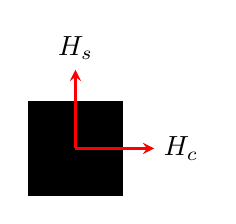
\begin{tikzpicture}[scale=2]
        \def\L{0.5}     %define arrow length
        \def\W{0.3}     %define arrow length
        \draw[fill=black] (\W,\W) rectangle (-\W,-\W);
        \draw[->,red,>=stealth,thick] (0  , 0) -- (\L,0);
        \draw (\L,0) node[anchor=west] {$H_c$};
        \draw[->,red,>=stealth,thick] (0, 0) -- (0,\L);
        \draw (0,\L) node[anchor=south] {$H_s$};
    \end{tikzpicture}
    \caption{Magnetometer showing $H_s$ and $H_c$}
    \label{fig:magAxisCross}
\end{figure}

\Cref{eq:magcross} shows the simplified equation for the magnetometer as described in \cite{AN215}. $V_b$ is the bridge voltage that is applied to the sensor. $S_s$ is the sensitivity in the sensitive direction. D is the cross field sensitivity offset. The HMC1052 datasheet\cite{HMC1052} mentions that the sensors have a bridge offset. The bridge offset is the sensor output when zero field is applied to the sensor and can be as large as \textpm1.25 Gauss. The bridge represented by $V_{os}$ in \cref{eq:magcross}.

\begin{equation}
    V_s = V_b \left(S_s H_s + D \cdot H_c + V_{os} \right)
    \label{eq:magcross}
\end{equation}
 
The bridge voltages are measured using an \ac{ADC} that uses the bridge voltage as its reference. To take this into account and simplify the equations, the following substitution is made:
\begin{equation}
    V_s'=\frac{V_s}{V_b}
    \label{eq:adcsub}
\end{equation}

\Cref{eq:magcross} is useful to determine the voltage that would be produced for a given magnetic field condition, but not the reverse when the sensor voltages are known but the fields are not.

Because the calculated field in the sensitive direction also depends on the field in the cross axis direction, \cref{eq:magcross} was duplicated for the cross field sensor voltage and both equations were solved simultaneously. This resulted in twice as many constants as \cref{eq:magcross}. The voltages $V_s'$ and $V_c'$ are the normalized \ac{ADC} voltages in the sensitive and cross axis respectively. Each of the constants from \cref{eq:magcross} has similar duplicate forms that comes from the extra equation that was used to solve for $H_s$. To distinguish the constants additional subscripts have been added. \Cref{eq:magsolved} shows \cref{eq:magcross} solved for the unknown quantity, $H_s$.

\begin{equation}
    \begin{split}
    H_s = & \frac{V'_s }{{S_s}_s - \frac{D_s \cdot D_c}{{S_s}_c}} - \frac{D_s \cdot  V'_c }{{S_s}_c \cdot {S_s}_s - D_s \cdot D_c}\\
    & {}- \frac{{S_s}_c \cdot {V_{os}}_s  -D_s \cdot {V_{os}}_c}{{S_s}_c \cdot {S_s}_s - D_s \cdot D_c}
    \end{split}
    \label{eq:magsolved} 
\end{equation}

\Cref{eq:magsolved} can be used to calculate the magnetic field from measured voltages, but the relationship between the constants is complex. To simplify \cref{eq:magsolved} the constants can be consolidated to get \cref{eq:magcal}.

\begin{equation}
    \label{eq:magcal}
    \begin{split}
        H_s &= C_1 \cdot V_s' + C_2 \cdot V_c' + C_3\\
        H_c &= C_4 \cdot V_s' + C_5 \cdot V_c' + C_6
    \end{split}
\end{equation}

In this case $V_s'$ and $V_c'$ are the \ac{ADC} values for the cross and sensitive axes, respectively. $C_1$, $C_2$, $C_4$, and $C_5$ are the sensitivity in the sensitive and cross directions and $C_3$ and $C_6$ correct for the bridge offset of the sensor and also compensates for external offsets. These offset values are used to correct for the torquer offsets.

\subsubsection{Magnetometer Calibration}
\label{sec:magcal}

To calibrate the magnetometer, the coefficients in \cref{eq:magcal} must be calculated. The magnetometer is first placed inside the Helmholtz Cage. The field is set under \matlab control so the entire calibration process can run automatically. The calibration program sweeps the field inside the Helmholtz Cage through a predefined sequence and reads the sensor output at each point. 
http://feeds.thisamericanlife.org/~r/talpodcast/~5/7S0vlAUUcfQ/532.mp3
The method of least squares is used to solve \cref{eq:magmat} for the coefficients in \cref{eq:magcal}. Each line in the $\matt{A}$ matrix represents a separate magnetic field measurement. $H_n$ is the $n^{\text{\tiny th}}$ value set by the Helmholtz cage in the sensitive axis. 

\begin{equation}
    \label{eq:magmat}
    \begin{split}
    \vect{b}&=\matt{A} \vect{x} \\
    {\text{\raggedright where}} \\
    \vect{b}&= 
    \begin{bmatrix}
        H_1 \\
        \vdots \\
        H_n \\
    \end{bmatrix} \\
    \matt{A}&=
    \begin{bmatrix}
        {V_s}_1 & {V_c}_1 & 1 \\
        \vdots & \vdots & \vdots\\
        {V_s}_n & {V_c}_n & 1 \\
    \end{bmatrix} \\
    \vect{x}&= 
    \begin{bmatrix}
        C_1 \\
        C_2 \\
        C_3 \\
    \end{bmatrix} 
    \end{split}
\end{equation}

The least squared solution minimizes the error across all data points. This results in calibration values that minimize error across the range of calibration points that were taken. This means that the points used to do the calibration should span the range of values that the magnetometer is expected to measure. 

\subsection{\acs{MEMS} Gyros}

For flight, a LPY410AL \ac{MEMS} gyro will also be used to sense rotation rates. \ac{MEMS} gyros have limited resolution compared to what can be achieved with the magnetometer. The LPY410AL has a maximum range of \textpm 400\textdegree /sec. The LPY410AL has a zero-rate sensitivity drift of 0.03~dps/\textdegree C. The desired rotation rate of the satellite is about 500~\textmu dps. This means that for a 1\textdegree C temperature change the rotation rate could change by 58 times the desired rotation rate. The LPY410AL also has a rate noise density of 0.014~$\unit{dps}{/}\sqrt{\unit{Hz}}$ so even at a slow sample rate of 1~Hz, the noise is 27,000 times larger than the desired rotation rate.

\ac{MEMS} gyros do, however, give good results if the rotation rates are large, such as after the satellite is ejected from the \ac{PPOD}. If the satellite is rotating fast enough, the magnetometer readings will alias and it can appear that the satellite is rotating at a speed that is much less than the actual speed. If the rotation rates are too high for the \ac{MEMS} gyro, the output will saturate and while the rotation rates are not measurable a direction and lower bound can be determined.


\section{Embedded System}

At the heart of the \ac{ACDS} is an embedded system. This system is responsible for running the algorithm, taking housekeeping data and, interfacing with the rest of the satellite.

\subsection{Processor}

The processor used for the \ac{ACDS} and all systems on \ac{ARC} is the Texas Instruments MSP430F2618. The MSP430 is a microcontroller aimed at low power applications. The MSP430f2618 runs at a maximum speed of 16~MHz and has 8~kB of \ac{RAM} and 116~kB of flash~memory. The MSP430 microcontrollers do not have an external memory bus so there is no way to add extra \ac{RAM} or flash~memory to the address space of the MSP430.

\subsection{SD card}

For flight data storage a SD card is used. This is necessary because of the needed space and write times. The internal flash is limited and also needs to be used for program storage making it undesirable for data storage. Furthermore, the internal flash can't be read while it is being written. Write times for the internal flash are fairly slow and require that the processor disable interrupts, making normal operation difficult. The flash shares the same address space as the \ac{RAM} and has the same access time. This makes the internal flash an attractive place to put settings and calibration data that are written few times but accessed often as any data on the SD card must be copied into \ac{RAM} before being used.

\subsection{\acs{ARC} Bus Communication}

The sensor data is read by the \ac{LEDL} board and sent over the bus to the \ac{ACDS} board. The \ac{ACDS} board initiates the connection by sending a command to tell how often measurements should be sent. The \ac{LEDL} then takes sensor data and sends it at the requested interval.

\begin{comment}
\section{Finished Board}

\Cref{fig:boardPhoto} shows the finished \ac{ACDS} board with torquers and pull pin. 

\begin{figure}[!ht]
    \centering
    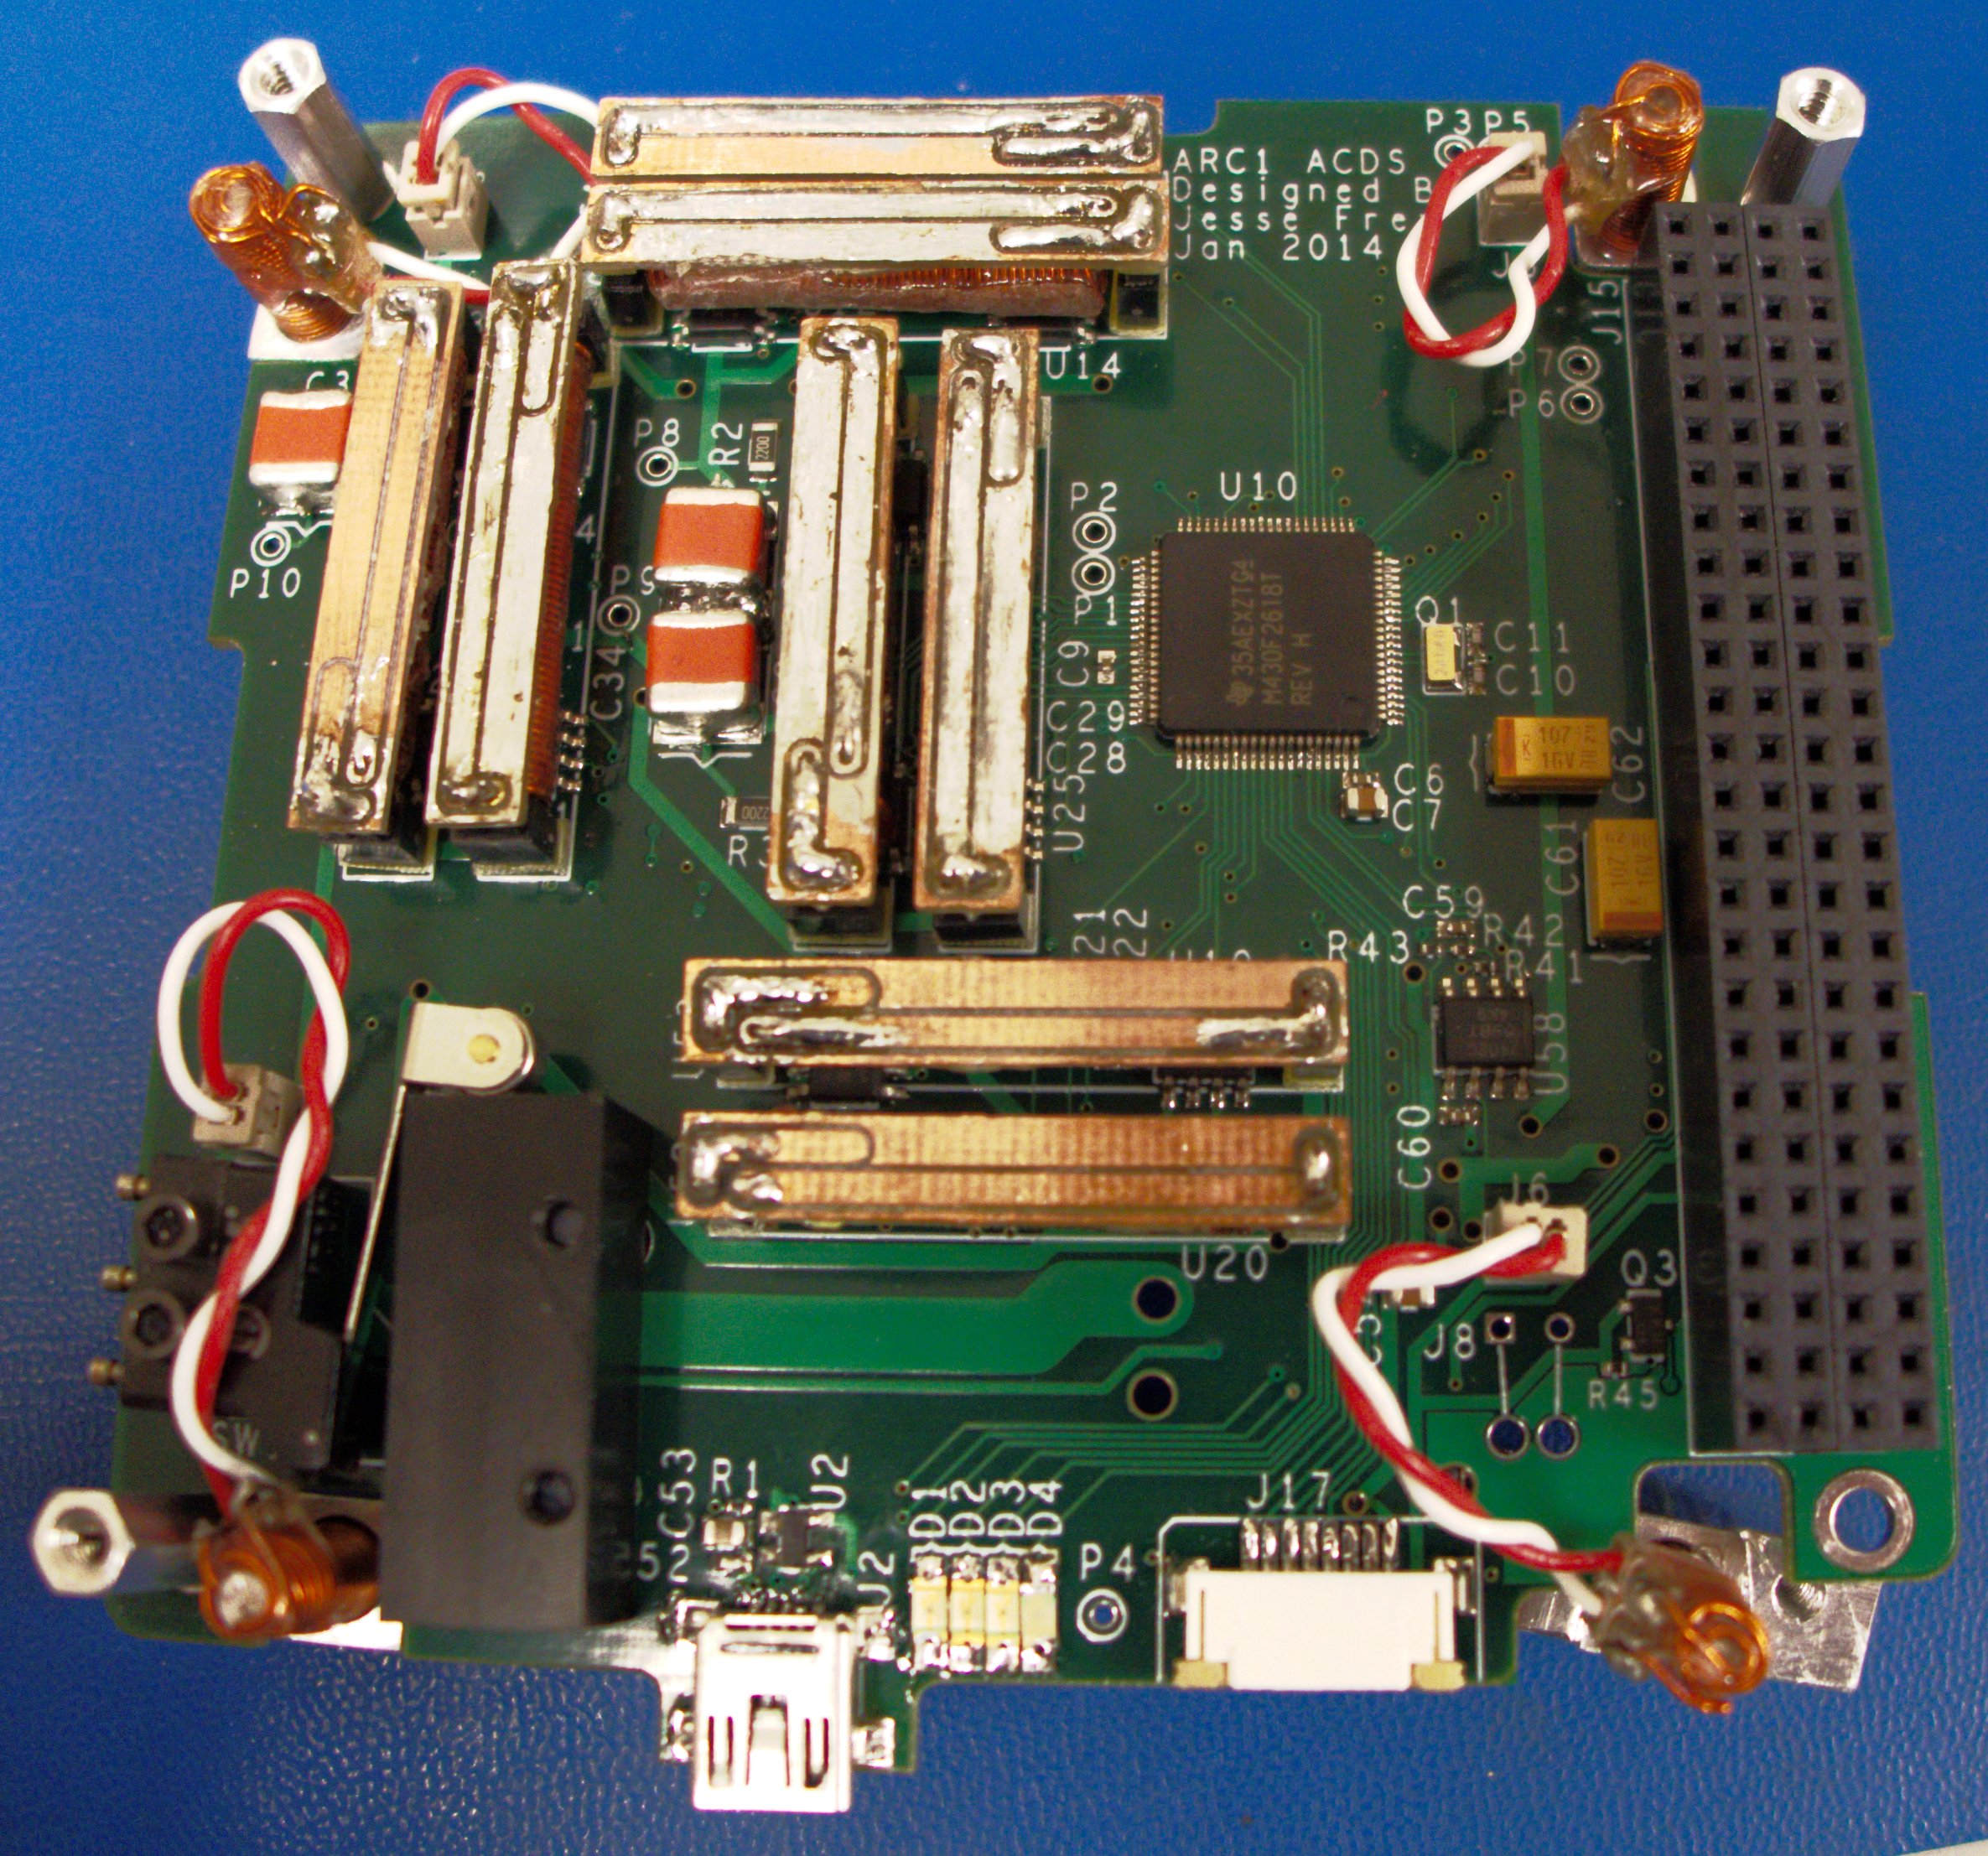
\includegraphics[width=0.5\linewidth]{ACDS-board-photo}
    \caption{The finished \ac{ARC} \ac{ACDS} hardware}
    \label{fig:boardPhoto}
\end{figure}
\end{comment}

\begin{comment}
\section{Board Layout}

\Cref{fig:3dview} shows the \ac{ACDS} system. The X and Y axis torquers are shown on the board as well as the pull pin and header. The header and pull pin locations are more or less fixed which doesn't leave much wiggle room for where to place the torquers.

\begin{figure}[H]
    \centering
    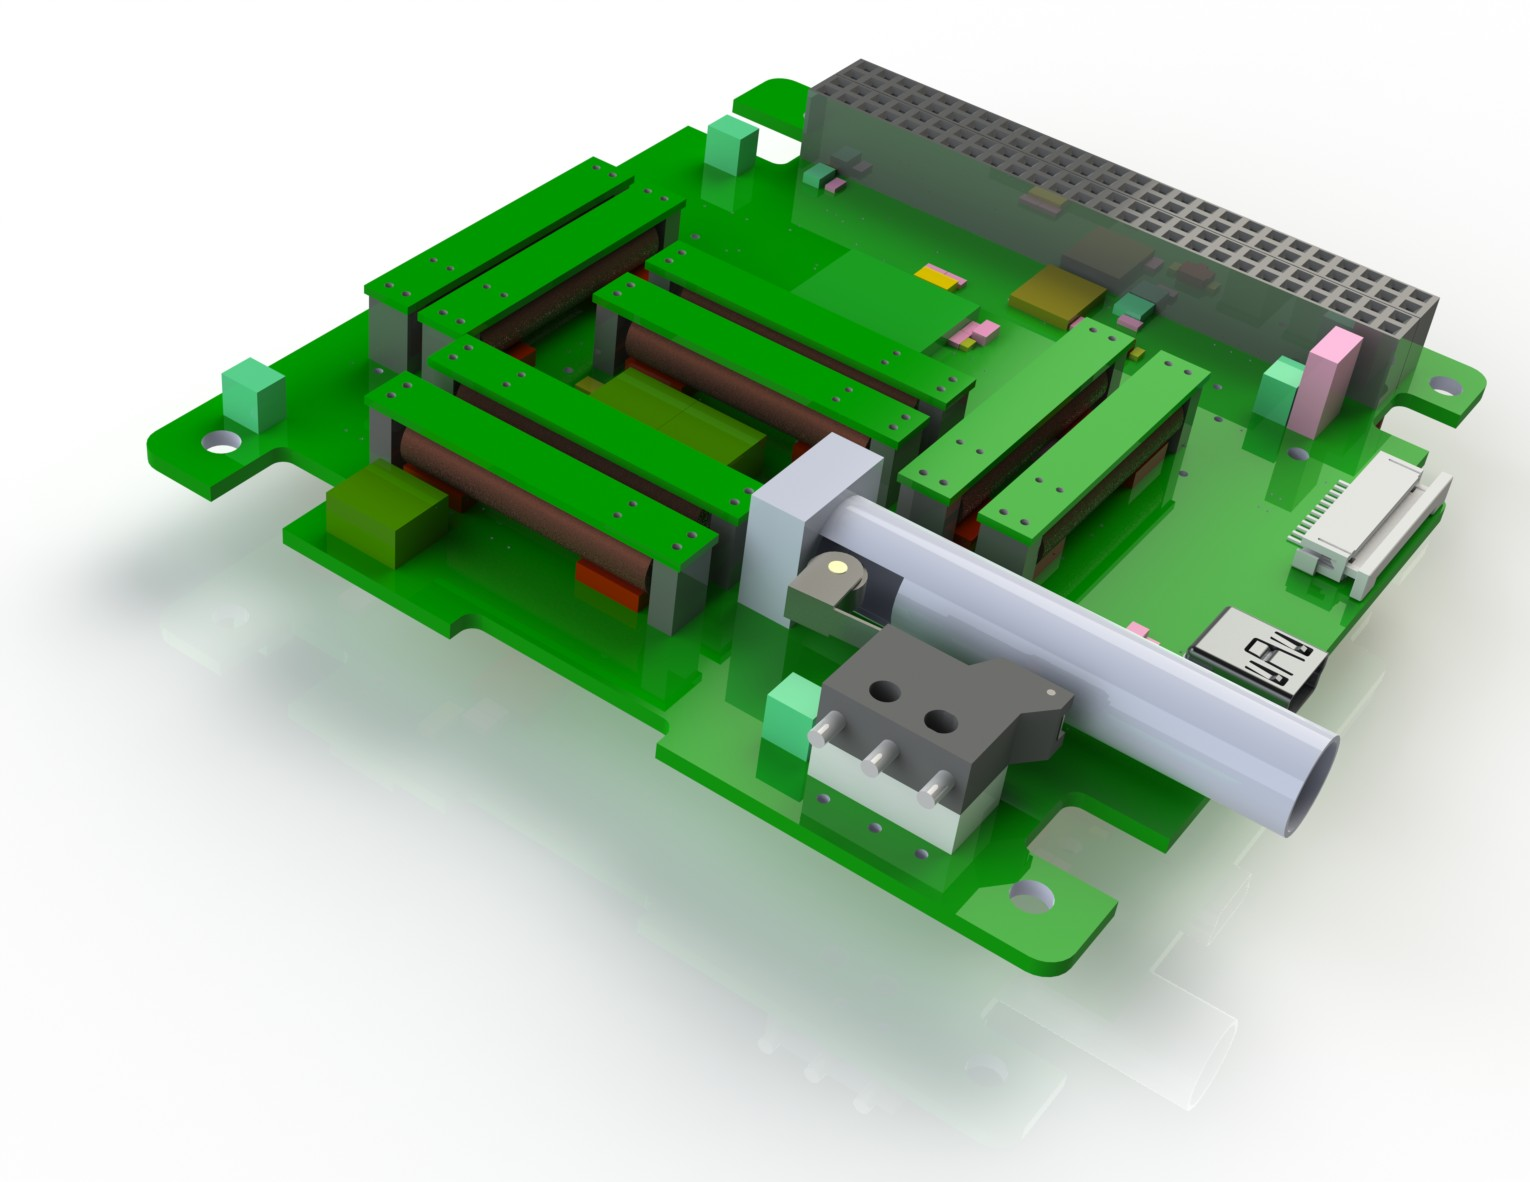
\includegraphics[width=\textwidth]{board-drawing}
    \caption{3D view of the CubeSat \acs{ACDS} system}
    \label{fig:3dview}
\end{figure}

\end{comment}

\begin{comment}
\begin{figure}[H]
    \centering
    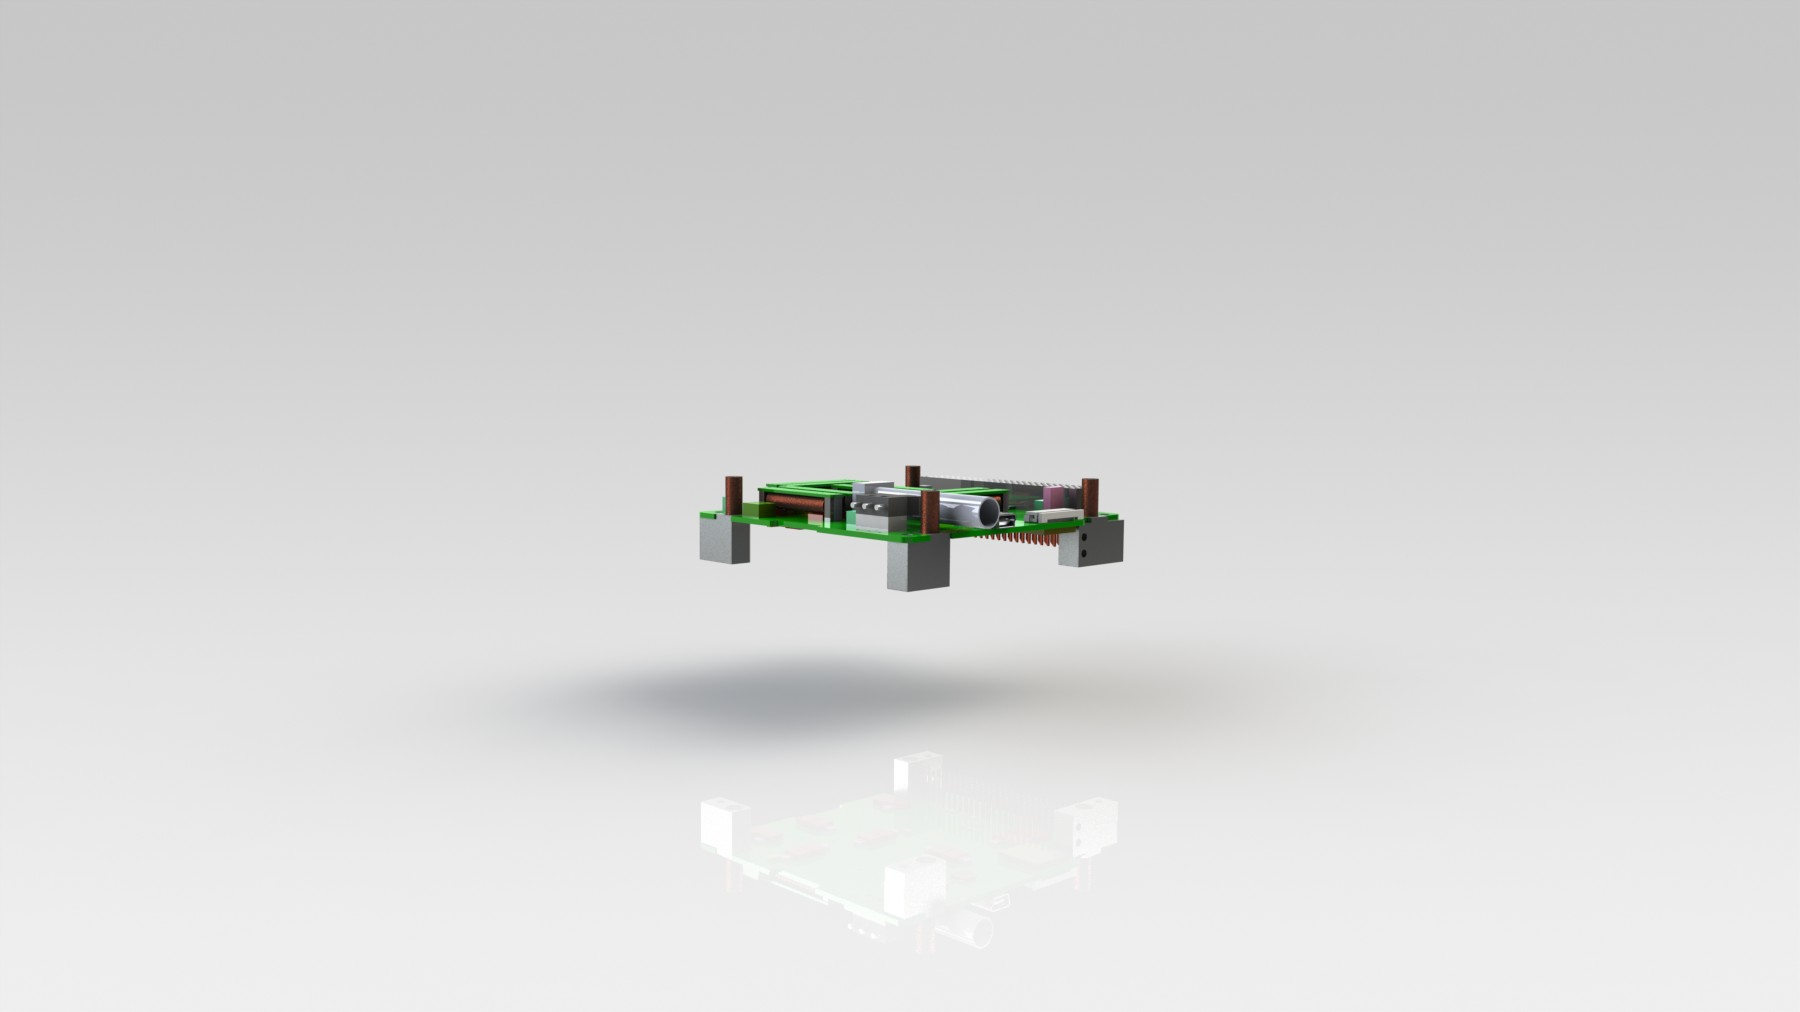
\includegraphics[width=\textwidth]{board-drawing-with-standoffs}
    \caption{3D view of the CubeSat \acs{ACDS} system with Z-axis torquers}
\end{figure}
\end{comment}

\begin{comment}

The \ac{ACDS} board is a four layer board with the inner layers as power and ground planes. \Cref{fig:layout} shows the \ac{PCB} layout for the \ac{ACDS} board. The circuitry is very repetitive and this was used when the board was laid out. A quick switching time is desired and moderate currents are involved, the lines to and from the \acp{MOSFET} were kept as short as possible. The power plane is split so that there is a 3.3V plane underneath the MSP430 and a $V_{batt}$ plane elsewhere.

\begin{figure}[H]
    \centering
    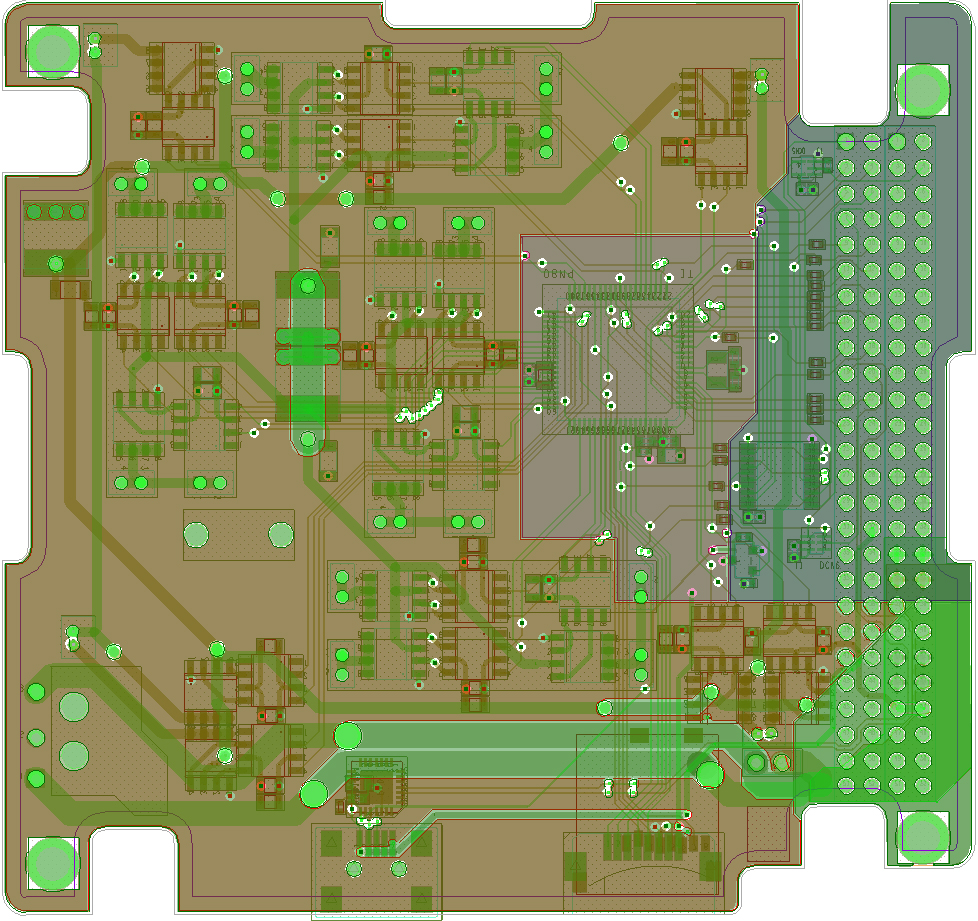
\includegraphics[width=\textwidth]{board-design}
    \caption{Board Layout for the CubeSat \acs{ACDS} system}
    \label{fig:layout}
\end{figure}

\end{comment}
